\documentclass[letterpaper, dvipsnames]{article}
\usepackage[utf8]{inputenc}
\usepackage[ngerman]{babel} % Package for translating default language into german e.g. table of contents - Inhaltsverzechnis 


\usepackage{graphicx} % Package for adding pictures
\usepackage{float} % Package for allowing to float images
\graphicspath{ {Pictures/} }

\usepackage{hyperref} % Package for adding urls
\usepackage{fancyhdr} % Package for manipulating header and footer

\usepackage[square, numbers, sort&compress]{natbib} % Package for table of contents
\bibliographystyle{unsrtnat}
\usepackage[nottoc]{tocbibind} % Package for adding References in the table of contents
\usepackage{listings} % Package for adding javascript code with code highlighting
\usepackage[dvipsnames]{xcolor} % Package for adding colors
\usepackage{textcomp} % Package for using arrows

\definecolor{purple}{rgb}{0.65, 0.12, 0.82}
\definecolor{main-color}{rgb}{0.6627, 0.7176, 0.7764}
\definecolor{back-color}{rgb}{0.1686, 0.1686, 0.1686}

\lstdefinelanguage{JavaScript}
{
  keywords = {typeof, new, true, false, function, return, null, switch, var, if, in, while, do, as, else, case, break, class, export, boolean, throw, implements, import, this, constructor, string, number, public, private, static, const, var, let, void, undefined},
  morekeywords = [2]{class, export, boolean, throw, implements, import, this, interface, async, await, for, any},
  morekeywords = [3]{Promise, Observable},
  morekeywords = [4]{log, prototype},
  otherkeywords = {;},
  comment = [l]{//},
  morecomment = [s]{/*}{*/},
  morestring = [b]',
  morestring = [b]",
}

\lstset
{
  language= JavaScript,
  commentstyle = {\color{OliveGreen}},
  stringstyle = {\color{OliveGreen}},
  keywordstyle = {\color{orange}\bfseries},
  keywordstyle = [2]{\color{orange}},
  keywordstyle = [3]{\color{Orchid}},
  keywordstyle = [4]{\color{TealBlue}},
  keywordstyle = [5]{\color{orange}},
  basicstyle = {\ttfamily \color{black}},
  backgroundcolor = {\color{white}},    
  sensitive = false,
  breaklines = true,
  showstringspaces= false,
  showtabs = false,
  showspaces= false,
  extendedchars= true
}

\begin{document}

\begin{titlepage}
\begin{minipage}{0.9\linewidth}
\begin{center}
\centering 
	      		 

\includegraphics[width=0.65\linewidth]{hm}
	
\begin{center}
\huge{\textsc{\scshape{ Bachelorarbeit}}}
\end{center}

\vspace{1cm}
{\scshape{\Large Vergleich von Sprachmitteln zur asynchronen Verarbeitung am Beispiel von Typescript\par}}
\vspace{1cm}
    
  
Verfasser  \linebreak
 {\Large Marco Leko\par}
 	\vspace{1.5cm}
angestrebter akademischer Grad\linebreak
 {\Large Bachelor of Science (BSc)\par}
	\vspace{1cm}

\flushleft
\begin{tabular}{ll}
München, 6. Februar 2019\linebreak

\vspace{1cm}&   \\
  Matrikelnummer: & 54442114 \vspace{0.3cm} \\ 
  Studienfach: & Wirtschaftsinformatik \vspace{0.3cm} \\
  Semester: & Wintersemester 2018/2019 \vspace{0.3cm} \\ 
  Betreuer: & Prof. Dr. Bastian Katz \\
 \end{tabular}

\end{center}
\end{minipage}
\end{titlepage}
\setlength{\headheight}{45pt}
\pagestyle{fancy}
\fancyhf{} % clear all header and footer fields
\rhead{
\includegraphics[width=2.8cm,height=1.3cm]{Hochschule_muenchen_logo.jpg}}
\lhead{Hochschule München}
\fancyfoot[C]{\thepage}
\thispagestyle{fancy}
\setcounter{secnumdepth}{0}
\section{Eidesstattliche Erklärung}

Hiermit versichere ich, die vorliegende Bachelorarbeit selbstständig und nur unter Verwendung der von mir angegebenen Quellen und Hilfsmittel verfasst zu haben. Sowohl inhaltlich als auch wörtlich entnommene Inhalte wurden als solche kenntlich gemacht. Die Arbeit hat in dieser oder vergleichbarer Form noch keinem anderem Prüfungsgremium vorgelegen.
\\[1.5cm]
Datum:	\hrulefill\enspace Unterschrift: \hrulefill


\newpage

\section{Danksagungen}
**Meine Danksagung**

\tableofcontents
\setcounter{secnumdepth}{1}

\section{Einführung}

Javascript ist im Aufwind mehr denn je. Sie ist die meist genutzte Programmiersprache unter Entwicklern. Laut der diesjährigen Umfrage von Stackoverflow belegte sie zum sechsten mal in Folge den ersten Platz\cite{programming-language-survey}. Doch woher kommt dieser Erfolg? \\

\noindent
Wenn es um das Web geht, war Javascript als Skriptsprache schon immer Vorreiter. Doch diese Sprache hat seine Stärken auch in der Vielfalt seiner Einsatzmöglichkeiten. Wie mit dem Framework Node.js, dass ab 2009 in Erscheinung getreten ist, war es möglich Server-seitigen Javascript-Code zu implementieren. Dies hatte zur Folge, dass man sich nicht mit multiplen Programmiersprachen auseinandersetzen musste. Man hatte eine Vereinheitlichung in seiner Code-Basis gefunden. Zudem bietet Node.js mit npm als Paketmanager die größte Auswahl an Open-Source-Libraries. Ein weiterer Punkt ist die Multi-Plattform-Kompatibilität die Javascript z.B. mit Angular offenbart. Mit diesem Framework kann man mit einer Code-Basis sowohl Web-Anwendungen als auch Apps für mobile Geräte entwickeln. Diese Hybrid Applikationen werden Progressive Web Apps genannt und können durch optimiertes Caching auch im Offline Modus betrieben werden. Das ist nur möglich, da Javascript's Ausführung vom Betriebssystem unabhängig ist. Und genau das bietet auch Typescript. Da Typescript ein \textit{Superset} von Javascript ist, kann jeder Javascript Code auch in Typescript interpretiert werden. Der Unterschied von Typescript zu Javascript ist die statische Typisierung. Das bedeutet, dass Variablen, Methoden und Funktionsparameter im Vorfeld mit einem Typ versehen werden. Aufgrund dessen können Bugs zur Laufzeit schneller erkannt werden. Zudem lässt sich der Code durch die Kapselung in Objekten leicht modular aufbauen und dokumentieren.\\

\noindent
Doch mit der Vielfalt steigt auch die Komplexität der Sprache. Schon zum vierten Jahr in Folge erschien eine neue Version von Javascript, die neueste Features mit sich bringt. Beispielsweise ermöglichen Promises und async await einen weiteren Ansatz zur asynchronen Verarbeitung. Somit werden Applikation, die ereignisgesteuert operieren, neue Möglichkeiten geboten. Mit Callbacks, Promises und Streams bekommen Entwickler verschiedene Optionen der asynchronen Datenverarbeitung zur Verfügung. Die Einsatzmöglichkeiten in einem Projekt können variieren, jedoch welcher Ansatz in welcher Situation sinnvoller erscheint, ist besonders für Entwickler mit wenig Erfahrung schwer zu erkennen.

\subsection{Zielsetzung}

Ziel der Arbeit ist es die Betrachtung und Aufbereitung des Einsatzes von Sprachmitteln zur asynchronen Verarbeitung in Typescript in einer Form, die Einsteigern in die Thematik hilft, die unterschiedlichen Konzepte voneinander abzugrenzen und richtig einzusetzen. Dazu soll asynchrone Verarbeitung insgesamt anhand brauchbarer und für den Einsatz von Typescript typischer Szenarien motiviert werden. Es werden die zur Verfügung stehenden Sprachmittel wie Callbacks, Promises und Observables mit ihren jeweiligen Features vorgestellt. Nach dem Lesen dieser Arbeit soll der Leser ein gewisses Verständnis dafür gewonnen haben, welche der vorgestellten Sprachmitteln für welchen Anwendungsfall besser geeignet ist.\\

\noindent
Zielgruppe dieser Arbeit sind Personen, die Grundkenntnisse in der Sprache Javascript/Typescript vorweisen können. Des Weiteren sollte man von dem Modell der asynchronen Datenverarbeitung wie Callbacks, Promises und Oberservables schon mal gehört haben, da diese in der Arbeit gegenübergestellt werden.

\subsection{Aufbau}

In dieser Arbeit werden die jeweiligen Ausarbeitungen der Ansätze mit Code-Beispielen unterstützt. Neben simulierten Anwendungsbeispielen zum Einstieg werden auch praxisnahe Beispiele wie z.B. Aufrufe an einer REST-API dargestellt. Das Code-Projekt lässt sich fachlich in den Modulen Callbacks, Promises, Async Await und RxJS unterteilen. Die Module haben jeweils eine introduction.ts Datei zur Einführung, eine stories.ts Datei, die entweder Funktionen oder Klassen anbietet und eine stories-usage.ts Datei, die diese Klassen oder Funktionen ausführt. In den jeweiligen Sektionen wird separat gezeigt, wie die einzelnen Dateien ausgeführt werden. Das Repository für das Projekt ist zu finden unter: 

\begin{center}
\url{https://github.com/MarcoLeko/async-patterns.git}
\end{center}

\noindent
Zu beachten ist, dass vor dem Ausführen des Projektes \textbf{Node.js} auf dem Rechner installiert sein muss, um den integrierten Paket-Manager \textbf{npm} nutzen zu können. Da \textbf{RxJS} nicht von vornherein von Javascript mitgeliefert wird, wird eine sog. \glqq Third-Party Library\grqq{} dafür benötigt. Sobald npm installiert ist, muss in dem Stammverzeichnis des Projekts \textbf{npm install} ausgeführt werden, um die jeweiligen Libraries herunterzuladen. Node.js kann man unter folgendem Link herunterladen:

\begin{center}
\url{https://nodejs.org/en/}
\end{center}

\section{Grundlagen}

\subsection{Typescript}
Typescript. Bereits der Name sagt schon was diese Sprache ausmacht. Sie ist eine typisierte Form der Skriptsprache Javascript. Besonders Javascript-Entwickler sträubten sich Anfangs mit der Sprache auseinanderzusetzen. Die Stärke von Javascript liegt in ihrer Flexibilität und der Tatsache nicht mehr code schreiben zu müssen als man braucht. Doch den Kompromiss den man mit Typescript eingeht, zahlt sich am Ende mit dem Zuwachs der Projektgröße aus. Da der Typescript Kompiler bereits Fehler beim Kompilieren erkennt, stellt sich die Frage, ob man lieber Fehler beim Entwickeln oder in der Produktion eines Projekts entdecken möchte. Dabei ist das \textbf{Tooling} der größte Vorteil von Typescript. Wenn man mit Typ-Annotationen oder mit Libraries, die streng typisiert sind, arbeitet, wird der Code von der Entwicklungsumgebung automatisch dokumentiert. Das heißt beim Entwickeln mit einem Code-Editor wird nicht zusätzlich verlangt, die Dokumentation der benötigten Library zu öffnen, um jeden einzelnen Rückgabetyp der Methode zu sehen. Wenn man nun von einem reinen Javascript-Hintergrund kommt, gibt es so gut wie keine Lernkurve die Sprache zu bewältigen. Das liegt daran, dass jeder valide Code von Javascript auch in Typescript ausführbar ist. Der Lernprozess steigt mit zunehmender Nutzung.

\subsubsection{Beispiel}

\begin{figure}[H]
\begin{lstlisting}[basicstyle=\small]
class Greeter {
    greeting: string;
    constructor (message: string) {
        this.greeting = message;
    }
    greet() {
        return "Hello, " + this.greeting;
    }
}  
\end{lstlisting}
\caption{Typescript Klasse \cite{typescript-example}}
\end{figure}

\begin{figure}[H]
\begin{lstlisting}[basicstyle=\small]
var Greeter = (function () {
    function Greeter(message) {
        this.greeting = message;
    }
    Greeter.prototype.greet = function () {
        return "Hello, " + this.greeting;
    };
    return Greeter;
})(); 
\end{lstlisting}
\caption{Überführung in Javascript \cite{typescript-example}}
\end{figure}

\noindent
Typescript selbst kann nicht selbständig ausgeführt werden. Das heißt in einem Browser oder auf einem Server wird unter Umständen immer noch Javascript genutzt. Mit dem Typescript Compiler werden daher Dateien mit dem Suffix *.ts in *.js überführt. Im oberen Code-Schnipsel wurden die Variablen und die Klassenmethoden nach Typescript-Standard deklariert. Diese Typen werden beim transpilieren in Javascript ignoriert. Der Kompiler prüft dann, ob beim übergeben eines Parameters in den Konstruktor ein String Wert eingesetzt wird. Wenn nicht, wird dies als ein Fehler erkannt. In der vom Kompiler auf Javascript übersetzten Version werden die erstellten Klassen und Typen vollständig eliminiert. Was verbleibt ist die Übersetzung der Methode greet() und des Konstruktors. Zudem werden auch nicht direkt deklarierte (implizite) Typen übersetzt. Wie in diesem Fall wird erkannt, dass die Methode greet() ein Wert vom Typ String zurückgibt. Ungleich wie mit Java oder C\# gewährleistet Typescript aus der streng typisierten Welt rauszufahren.

\begin{figure}[H]
\begin{lstlisting}[basicstyle=\small]
let count: any = 23;

count = 'Oops transformed to string!'
\end{lstlisting}
\caption{Wenn unbekannte Objekte von einem API-Aufruf verarbeitet werden, können diese als any deklariert werden.}
\end{figure}

\noindent
Der Kompiler würde hierbei keinen Fehler anzeigen. Obwohl im Idealfall auf die \textbf{any} Notation verzichtet werden sollte, wird dennoch Javascripts Flexibilität geboten. 

\subsubsection{Kompiler}
Ein großer Vorteil von Typescript ist die Möglichkeit auf verschiedene Javascript/Ecmascript Version zu transpilieren. Wenn bestimmte Browser Javascripts neueste Feature noch nicht unterstützen, kann das Kompilat auf ältere Ecmascript Versionen übersetzt werden. Diese Konfiguration wird mit Hilfe einer \textbf{tsconfig.json} Datei bewältigt. Die Auflistung einer solchen Datei zeigt, dass es sich um das Stammverzeichnis des Projekts handelt. Hier können die Kompiler-Optionen für Typescript gesetzt werden oder Dateien von der Übersetzung ein- oder ausgeschlossen werden. Ein Beispiel für die Konfiguration einer solchen Datei könnte wie folgt aussehen: 

\begin{figure}[H]
\begin{lstlisting}[basicstyle=\small]
{
  "compilerOptions": {
    "target": "esnext",
    "module": "commonjs",
    "lib": ["dom", "es2018"],
    "typeRoots": [
      "node_modules/@types"
    ]
  }
}
\end{lstlisting}
\caption{Auflistung einer tsconfig.json Datei}
\end{figure}

\noindent
Mit dem Wert “target” wird die ausgeführte Javascript Version eingestellt. Wenn der Wert nicht bestimmt ist, wird standardmäßig nach es3 übersetzt. Um stets die aktuellste Version zu nutzen, wird für das Projekt \textbf{esnext} angegeben. Typescript wird im Terminal unter dem Verzeichnis einer Typescript-Datei mit \textit{tsc Dateiname.ts} kompiliert. In den für diese Arbeit genutzten Code-Beispielen werden die Startskripte von npm ausgeführt.

\begin{figure}[H]
\begin{lstlisting}[basicstyle=\small]
  ...
  "scripts": {
    "start": "webpack --watch",
    "build": "webpack"
  },
  ...
\end{lstlisting}
\caption{Auflistung ist unter der \textbf{package.json} Datei zu finden}
\label{npm-ex-script}
\end{figure}

\noindent
Wie man in Abbildung \ref{npm-ex-script} sehen kann, führt \textbf{npm run start} nicht tsc aus, sondern \textbf{webpack --watch} aus. Webpack ist ein sog. \textbf{Module-Bundler}. Das Projekt ist nicht nur fachlich, sondern auch technisch in Modulen gegliedert. Diese Module sollten nach Möglichkeit einzeln ausgeführt werden. Ein Module-Bundler läuft während des Build-Prozesses und erfüllt im Wesentlichen zwei Aufgaben. Den Code mit dem Typescript-Kompiler in Javascript zu transpilieren und die daraus resultierenden Kompilate in einer zentralen Datei (main.js) zu bündeln. Um das zu erreichen, nimmt Webpack eine Eingangsdatei als Einstiegspunkt an und bündelt den Inhalt inklusive aller involvierten Importe. Welchen Mehrwert hat Webpack also für das Projekt? \\

\noindent
Beim Ausführen der Beispiele muss nicht jedes mal die jeweilige TS-Datei in eine JS-Datei überführt und das erstellte Kompilat daraufhin in die HTML-Datei referenziert werden. Die HTML-Datei hat nur das Bündel main.js als Referenz und je nach definiertem Einstiegspunkt in der \textbf{webpack.config.js} wird ein neues Bündel erzeugt. Mit der Einstellung \textbf{--watch} werden Veränderung des Codes in Echtzeit kompiliert. Sollten nun Änderungen im Code vorgenommen werden, erstellt Webpack ein neues Bündel. Nach dem Kompilieren muss nur noch die HTML-Seite geöffnet/aktualisiert werden. Um mehr von Typescript und dessen Nutzung mit Webpack zu erfahren, findet unter folgendem Link mehr dazu:

\begin{center}
\url{https://webpack.js.org/guides/typescript/} 
\end{center}

\subsection{Terminologie}

Um die Abgrenzung von verschiedenen asynchronen Sprachmitteln zu beherrschen, muss vorerst geklärt werden, was Asynchronität bedeutet.\\

\noindent
Der zentrale Teil eines Computers, welches Programme und einzelne Schritte zum Ausführen bringt, ist der Prozessor. Die Geschwindigkeit in der eine Schleife von einem Programm ausgeführt wird, hängt von der Geschwindigkeit des Prozessors ab. Programme interagieren jedoch mit Operationen außerhalb des Zuständigkeitsbereiches eines Prozessors, wie z.B. die Kommunikation über ein Netzwerk oder das Abfragen von Daten von der Festplatte. Solche Operationen hängen von anderen Ressourcen ab und brauchen Zeit. In solchen Szenarien wäre es unvorteilhaft, wenn der Prozessor, anstatt andere Operationen in der Zwischenzeit auszuführen, im Leerlauf stecken würde. Genau für solche Aufgaben ist das Betriebssystem da. Das Betriebssystem sorgt dafür, dass Kapazitäten des Prozessors auf parallel laufende Programme wechselt, während es auf die Antwort von ausgeführten Operationen wartet. Es entstehen dabei verschiedene \glqq Threads\grqq{}. Und hier kommt die Asynchronität ins Spiel:

\subsubsection{Asynchronität}

Ein \textbf{asynchrones} Programmiermodell erlaubt multiple Abläufe zum selben Zeitpunkt. Wenn eine Aktion ausgeführt wird, läuft das Programm in einem anderen \glqq Thread\grqq{} weiter. Sollte die Operation fertig gestellt sein, wird das Programm informiert und liefert das Ergebnis zurück. Ein Beispiel dafür wäre das Suchen von Dateien auf einer Festplatte\cite{asynchronitaet}.

\subsubsection{Synchronität}

In einem \textbf{synchronen} Programmiermodell entstehen Abläufe sequenziell. Wenn eine Funktion mit einer zeitintensiven Aktion abgerufen wird, wird das Ergebnis erst nach dem Beenden der Operation zurückgegeben. In diesem Zeitintervall werden keine Nebenoperationen ausgeführt\cite{asynchronitaet}.\\

\noindent
Man kann ein synchrones und asynchrones Modell mit einem kleinem Beispiel vergleichen: Eine Anwendung die zwei Ressourcen aus einem Netzwerk anfragt und die Ergebnisse miteinander kombiniert. In einer synchronen Umgebung würde man dies mit einem Funktionsaufruf nach dem anderen bewältigen. Das hat den Nachteil, dass die zweite Funktion erst dann ausführt, wenn die erste fertig ist. Die Gesamtzeit der Ausführung ist die Summe der Antwortzeiten der beiden Anfragen. Die Lösung dafür ist ein synchrones Programmverhalten mit mehreren kontrollierten Threads. Ein Thread ist ein Ausführungsstrang, der seine eigene Zeitleiste besitzt und innerhalb dieser Operationen ausführt. Ein zweiter Thread könnte zum selben Zeitpunkt die Funktion aufrufen und wenn beide Threads das Ergebnis geliefert bekommen resynchronisieren sie sich und kombinieren ihre Ergebnisse\cite{asynchronitaet}. Im folgenden Diagramm wird ein synchrones Modell mit einem Thread, mit zwei Threads und ein asynchrones Modell gegenübergestellt.

\begin{center}
\begin{figure}[H]
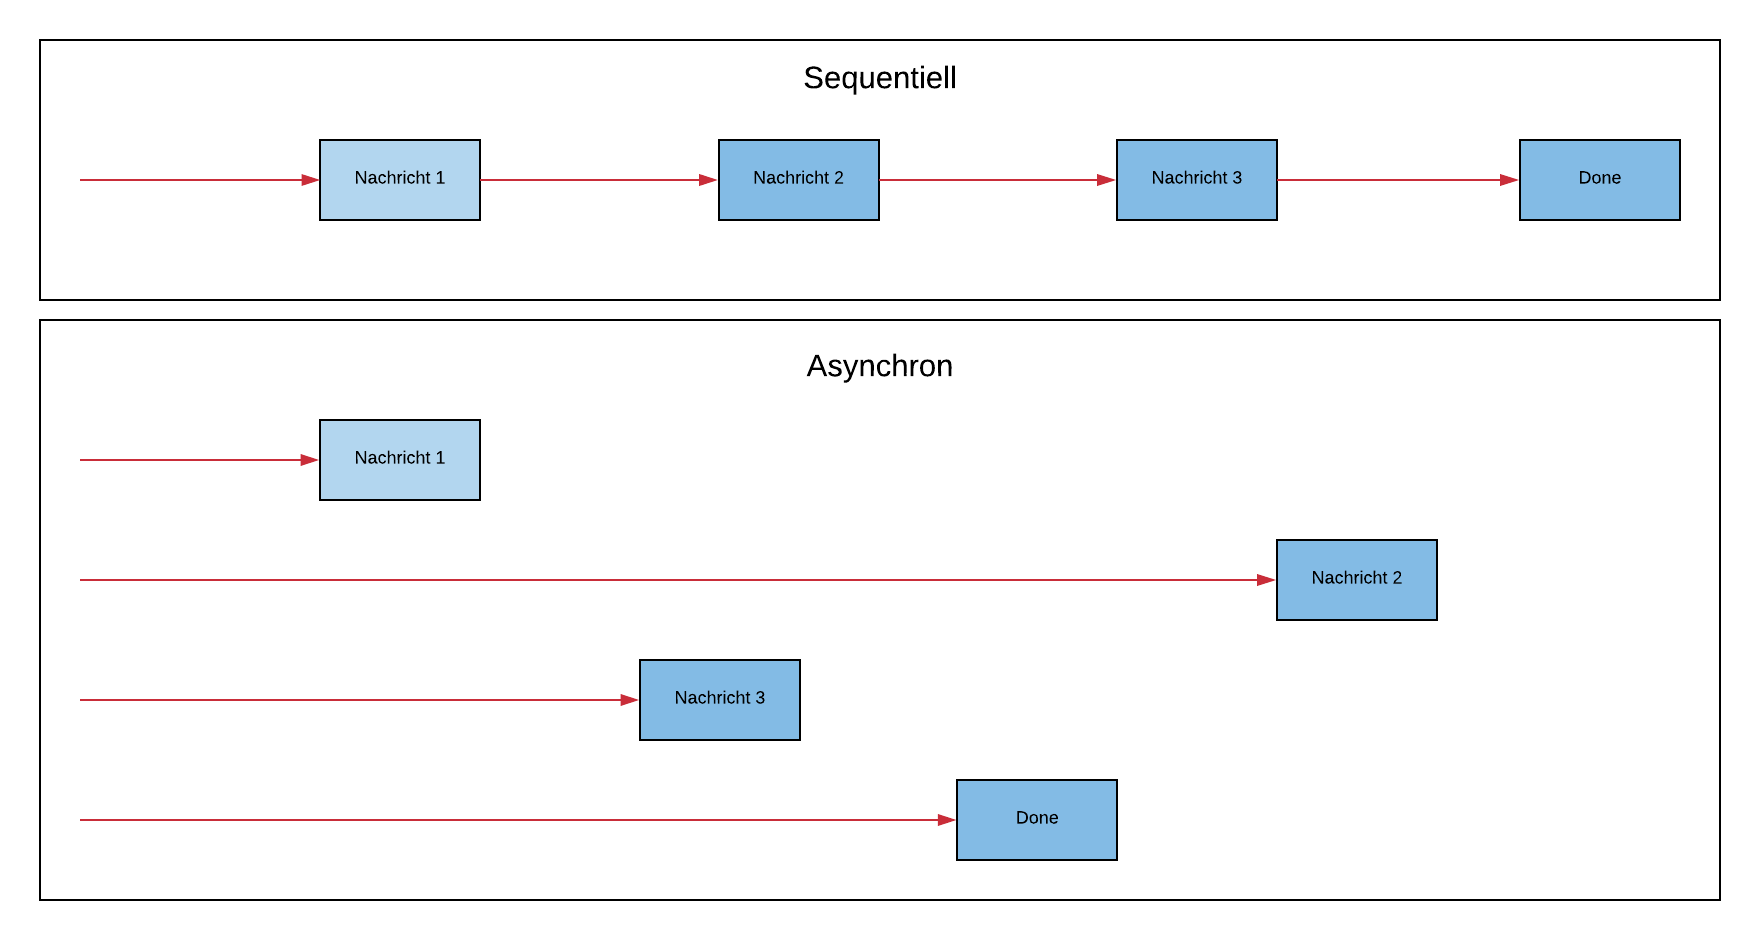
\includegraphics[width=12cm]{synchron-vs-asynchron-diagram}
\caption{Die blauen Linien repräsentieren die Zeit, in der das Programm ausführt und die roten Linien repräsentieren die Zeit, in der auf die Antwort gewartet wird.}
\end{figure}
\end{center}

\noindent
Im synchronen Modell ist die Zeit der Netzwerkanfrage ein Teil der Zeitleiste. Im asynchronen Modell hingegen führt das Starten einer asynchronen Operation zu einer neuen Zeitleiste. Zusammenfassend kann man also sagen, dass in dem synchronen Modell implizit auf die Aktionen gewartet wird, und in dem Asynchronen explizit.
\section{Callbacks}
Javascript ist eine ereignisgesteuerte Programmiersprache. Das bedeutet, anstatt auf blockierenden Code zu warten, führt Javascript Operationen weiter aus und reagiert wenn die Aktion fertig ist. Um sicherzustellen, dass Javascript abhängige Funktionen erst nach der Fertigstellung von asynchronen Operationen ausführt, wurde das Prinzip der \textbf{Callbacks} eingeführt. Doch wie regelt der Browser in welcher Reihenfolge der Code ausgeführt wird?

\subsection{Javascripts Laufzeitkonzept}
Dazu muss im groben das Verhalten des Javascript-Interpreters erklärt werden. Die wichtigsten Komponenten eines Javascript-Interpreters ist der Call stack und die Event Loop.\\

\noindent
Wenn ein Skript eine Funktion \textit{f} aufruft, fügt der Interpreter die Funktion zum Aufrufsstapel \textit{(Call stack)} hinzu. Wird nun eine Funktion \textit{g} innerhalb von \textit{f} aufgerufen, wird die innere Funktion weiter oben in den Call stack hinzugefügt. Wenn die Ausführung von \textit{f} fertig ist, wird diese Funktion aus dem Stapel entfernt und die Funktion, die sich weiter oben befindet, aufgerufen. Der Call stack verfolgt das Lifo-Prinzip (Last in - first out)\cite{javascript-interpreter}. Vor dem Ausführen des Beispiels muss folgend konfiguriert werden:

\begin{center}
    async-patterns$\,\to\,$ webpack.config.js
\end{center}

\begin{figure}[H]
\begin{lstlisting}[basicstyle=\small]
module.exports = {
    mode: 'development',
    entry: './src/modules/callbacks/introduction.ts',
    ...
}
\end{lstlisting}
\caption{Die webpack.config.js Datei befindet sich im Hauptverzeichnis des Projekts.}
\end{figure}

\begin{figure}[H]
\begin{lstlisting}[basicstyle=\small]
function h(z: string): void {
    console.log(z);
    console.log(new Error().stack); // (A)
}

function g(y: string): void {
    h(y + 'c'); // (B)
}

function f(x: string): void {
    g(x + 'b'); // (C)
}

f('a'); // (D)
\end{lstlisting}
\caption{Nutzung von abhängigen Funktionen in einem synchronen Programmiermodell.}
\end{figure}

\noindent
Anfänglich, wenn das Programm startet, ist der Call stack leer. Erst ab Zeile D mit dem Funktionsaufruf f('a') hat der Aufrufstapel einen Eingangspunkt. Der Einstiegspunkt befindet sich im globalen Geltungsbereich (\textit{global scope}):

\begin{itemize}
\item Globaler Geltungsbereich
\end{itemize}

\noindent
Nachdem die Funktion g(x + 'b') in Zeile C aufgerufen wurde, hat der stack zwei Eingangspunkte:

\begin{itemize}
\item Geltungsbereich innerhalb von Funktion \textit{f}
\item Globaler Geltungsbereich
\end{itemize}

\noindent
Nachdem Funktion h(y + 'c') aufgerufen wurden in Zeile B, hat der stack drei Eingangspunkte:

\begin{itemize}
\item Geltungsbereich innerhalb von Funktion \textit{g}
\item Geltungsbereich innerhalb von Funktion \textit{f}
\item Globaler Geltungsbereich
\end{itemize}

\noindent
Beim Ausführen des Codes zeigt die Konsole wie der Callstack vorgegangen ist:

\begin{figure}[H]
\begin{lstlisting}
abc
Error
    at h (stack_trace.js:2:17)
    at g (stack_trace.js:6:5)
    at f (stack_trace.js:9:5)
    at <global> (stack_trace.js:11:1)
\end{lstlisting}
\caption{Stellt die Anordnung der Aufrufe von unten nach oben dar.}
\label{stack-trace-error}
\end{figure}

\noindent
Javascripts Laufzeitkonzept lässt sich mit einem Warteschlangen-System vergleichen. Unabhängig davon wie zeitnah asynchrone Ereignisse wie timeouts oder Antworten aus einem Netzwerk ankommen, diese Prozesse werden erst in die Schlange gesetzt wenn der Stapel leer ist.

\begin{figure}[H]
\begin{lstlisting}[basicstyle=\small]
setTimeout(function() {
    console.log('second');
}, 10);

let num: number = 0;

while (num < 100000000) { // 100 Millionen Iterationen
    num = num + 1;
}

console.log('first');
// first
// second
\end{lstlisting}
\caption{Mit der setTimeout()-Funktion können Funktionsaufrufe verzögert werden.}
\label{First-timeout-example}
\end{figure}

\noindent
Eine Javascript Umgebung führt nur eine Aufgabe nacheinander aus. Während das Programm ausgeführt wird, läuft im Hintergrund eine Eventschleife, die eventuell eintreffende Ereignisse registriert. Diese Schleife wird auch als \textbf{Event Loop} bezeichnet. Im Beispiel von Abbildung \ref{First-timeout-example} wird die setTimout() Funktion genutzt. SetTimeout() ist eine WEB API Methode, die der Browser zur Verfügung stellt. Hierbei wird bestimmt mit welcher Verzögerung in Millisekunden die innere Funktion in den Callstack hinzugefügt wird. Um genau zu sein, wird die innere Funktion nicht direkt in den Call stack hinzugefügt. Die Eventschleife registriert, dass ein Ereignis nach einer Zeitverzögerung ausgelöst wurde, und sorgt dafür dass diese Funktion in den Callstack hinzugefügt wird, sobald dieser Leer ist. Wann auch immer ein Javascript Programm läuft, prüft die Event Loop ob ein neues Ereignis ausgelöst wurde\cite{regular-event-loop}.\\

\noindent
Um eine Funktion nach einer asynchronen Operation auszuführen, können Funktionen geschachtelt werden. Dazu wird eine Funktionen als Argument angenommen und erst dann aufgerufen, wenn eine blockierende Aktion fertig ist. Doch wie genau funktioniert diese Schachtelung von Funktionen?

\subsection{Funktionsweise}

Sowohl in Javascript als auch in Typescript sind Funktionen als Erste-Klasse-Objekte zu sehen. Aus diesem Grund können sie an Variablen gebunden oder als Argumente in anderen Funktionen oder als Rückgabewert übergeben werden. Diese übergebenen Funktionen heißen Callbacks.\\

\noindent
Callbacks, auch Rückruffunktionen genannt, bildet das Kernkonzept der \textbf{funktionalen Programmierung} in Javascript\cite{callbacks-intro}. In der funktionalen Programmierung sind Funktionen als Werte zu betrachten. Der Code besteht aus kleineren Funktionen, die in höher geordneten Funktionen eingesetzt oder miteinander kombiniert werden können (Komposition). Dadurch ist der Code wiederverwendbar und weniger fehleranfällig. Javascript bietet mit Arrays die Möglichkeit Callbacks sinnvoll einzusetzen.

\begin{figure}[H]
\begin{lstlisting}[basicstyle=\small]
const numbers: number[] = [1, 2, 3, 4, 5, 6];

function isEven(x): boolean { 
  return x % 2 === 0; 
}

const evenNumbers = numbers.filter(isEven);
console.log(evenNumbers) // 2 4 6
\end{lstlisting}
\caption{Die Funktion filter() gibt ein neues Array zurück.}
\label{callbacks-with-arrays}
\end{figure}

\noindent
Die Methode filter() nimmt Elemente eines Arrays heraus, basierend einer Funktion, die die Filterkonditionen bestimmt. Filter() ruft die Callback Funktion einmalig für jedes Element auf. Dabei wird zuerst, dass Element aus der Liste entnommen und dann die Kondition geprüft. Wenn also eine Funktion als Parameter übergeben wird, wird diese nicht sofort ausgeführt. Eine Funktion die ein Callback als Argument annimmt, wird auch höherrangige Funktion \textit{(Higher Order Function)} genannt\cite{callbacks-example}.

\subsection{Beispiel}
In den jeweiligen Sektionen wird das gleiche Praxisbeispiel, in verschiedenen Ausprägungen angewendet und gegenübergestellt. Mit der REST-API \textbf{JSONPlaceholder} wird ein Endpunkt für die Datenabfrage definiert. Hierbei handelt es sich um eine Open Source Endstelle, die Beispieldaten für das Prototyping oder zum Testen zur Verfügung stellt. Je nach Anwendungsfall werden verschiedene Ausführungen von Anfragen an diese Endstelle gemacht, um die Code-Beispiele so praxisnah wie möglich zu halten.\\

\noindent
Das folgende Beispiel richtet sich nach dem funktionalen Programmierparadigma, da durch die Nutzungen von \textbf{puren Funktionen}, das Callback Prinzip besser zur Geltung kommt. Eine pure Funktion, ist eine Funktion, die beim selben Input jedes mal das gleiche Output wiedergibt. Zu erwähnen ist jedoch, dass das Prinzip der Callbacks auch im objektorientiertem Schema umgesetzt werden kann. 

\begin{figure}[H]
\begin{lstlisting}[basicstyle=\small]
module.exports = {
    mode: 'development',
    entry: './src/modules/callbacks/stories-usage.ts',
    ...
}
\end{lstlisting}
\caption{Für die folgenden Beispiele sollte ../callbacks/stories-usage.ts als Eingangsdatei in die webpack.config.js definiert werden.}
\end{figure}

\begin{figure}[H]
\begin{lstlisting}[basicstyle=\small]
function makeRequest(url, onSuccess, onFailure?): void {
    const req = new XMLHttpRequest();
    req.open('GET', url);

    req.onload = () => {
        if (req.status === 200) {
            fakeLatency(() => onSuccess(JSON.parse(req.response));
        }
    };

    req.onerror = () => onFailure(Error('Network Error'));

    req.send();
}

function fakeLatency(callback): void {
    setTimeout(callback, 3000 * Math.random());
}

function baseUrl(): string {
    return 'https://jsonplaceholder.typicode.com/posts/';
}

function getAllChapters(onSuccess, onFailure?): void {
    makeRequest(baseUrl(), onSuccess, onFailure);
}

function getChapter(chapter, onSuccess, onFailure?): void {
    makeRequest(baseUrl() + chapter.toString(), onSuccess, onFailure);
}
\end{lstlisting}
\end{figure}

\begin{figure}[H]\ContinuedFloat
\begin{lstlisting}[basicstyle=\small]
function createElm(innerHTML): HTMLElement {
    const div = document.createElement('div');
    div.innerHTML = innerHTML;
    document.body.appendChild(div);
    return div;
}

function spawn(content: any): void {
    if (content instanceof Array === false) {
        content = [content];
    }
    content.forEach(elm => {
        const snippet = document.createElement('div');
        snippet.innerHTML = '<h1>${elm.title}</h1>
                             <div>
                                <i>${elm.id}</i>
                             </div>
                             <p>${elm.body}.</p>';

        document.body.insertBefore(snippet, loadingIcon);
    });
}

function catchError(err) {
     createElm('Ooops! Error Occurred! ${err}');
}

function displayFinished(): void {
    loadingIcon.style.display = 'none';
    createElm('All done!');
}

const loadingIcon = createElm('<svg>..</svg>');
\end{lstlisting}
\caption{Durch das funktionale Programmierparadigma verhindert man die Abhängigkeit von externen Variablen und umgeht somit unerwünschte Seiteneffekte.}
\end{figure}

\noindent
Dabei sind die wichtigsten Funktionen makeRequest(), getAllChapters(), getChapter() und spawn(). MakeRequest() führt eine Http-Anfrage gegen einen definierten Endpunkt aus. Wenn der Status der Antwort 200 beträgt, wird im Success-Callback vorangeschreitet. Bei einem Fehler wird der Error-Callback aufgerufen. Sowohl getAllChapter() als auch getChapter() führen makeRequest() aus, mit der Option im Erfolgs- und im Fehlerfall der Anfrage eine Aktion auszuführen. Spawn() nimmt ein Kapitel entgegen und lädt diesen in die DOM. Sollte ein Anwendungsfall sein, alle Kapitel der API anzufragen und bei Ankunft der Daten anzuzeigen, würde dies wie folgt aussehen:

\begin{figure}[H]
\begin{lstlisting}[basicstyle=\small]
getAllChapters(function(response) {
    spawn(response);
    displayFinished();
});
\end{lstlisting}
\caption{Zuerst wird der API-Aufruf ausgeführt und mit dem daraus resultierendem Objekt wird spawn() aufgerufen.}
\end{figure}

\noindent
In diesem Fall wird spawn() erst aufgerufen, wenn eine Antwort vom Endpunkt ankommt. Da Funktionen als Argument anderer Funktionen übergeben werden, können diese \glqq{}später\grqq{} innerhalb des Funktionsrumpfes aufgerufen werden \textit{(\glqq{}Call-back\grqq{})}. Um multiple asynchrone Operationen nacheinander auszuführen, müssen Funktionen ineinandergeschachtelt werden. So wird die Ausführung sequentiell fortgesetzt. Als Beispiel wird Kapitel eins bis drei chronologisch aufgerufen:

\begin{figure}[H]
\begin{lstlisting}[basicstyle=\small]
console.log('before execution');
getChapter(1, function(response1) {
    spawn(response1);
    getChapter(2, function(response2) {
        spawn(response2);
        getChapter(3, function(response3) {
            spawn(response3);
            displayFinished();
        });
    });
});
console.log('after execution');
\end{lstlisting}
\caption{Aktionen wie die Übertragung von Daten in einem Netzwerk finden in einem eigenen Thread statt.}
\end{figure}

\noindent
Auffallend in diesem Beispiel ist der Grad der Einrückung, der mit jeder weiteren asynchronen Operationen steigt. Der Ausführungsstrang sieht hier wie folgt aus aus:

\begin{enumerate}
    \item Console.log('before execution') wird ausgeführt.
    \item getChapter(1) wird ausgeführt.
    \item Die anonyme Funktion innerhalb von getChapter(1) wird erst aufgerufen, wenn das Objekt aus der Netzwerkanfrage ankommt. Alle darunter abhängigen Funktionen werden dementsprechend noch nicht aufgerufen.
    \item Console.log('after execution') wird ausgeführt. Der Call stack ist nun leer.
    \item Die Antwort ist angekommen. Die anonyme Funktion ruft spawn() auf.
    \item getChapter(2) wird aufgerufen.
    \item ...
\end{enumerate}

\noindent
Alle weiteren asynchrone Operationen innerhalb von getChapter(1) sind voneinander abhängig und bleiben innerhalb der selben Zeitleiste. Asynchronität ist ansteckend. Eine Funktion, die zur asynchronen Verarbeitung ein Callback nutzt, operiert selbst asynchron. Wenn nun ein Großteil eines Programms aus ineinandergeschachtelten Funktionen besteht, kann diese Struktur zur erhöhten Fehleranfälligkeit führen. Dank der sechsten Ecmascript Version können Pfeil-Funktionen in Javascript genutzt werden. Diese sind syntaktisch kürzer als anonyme Funktionen. Wenn nun die fehlgeschlagenen Callbacks zusätzlich verarbeitet werden sollen, dann würde dies so aussehen:

\begin{figure}[H]
\begin{lstlisting}[basicstyle=\small]
getChapter(1, response1 => { // (*)
    spawn(response1);
    getChapter(2, response2 => { // (**)
        spawn(response2);
        getChapter(3, response3 => { // (***)
            spawn(response3);
            displayFinished();
        }, err3 => catchError(err3)); // (***)
    }, err2 => catchError(err2)); // (**)
}, err1 => catchError(err1)); // (*)
\end{lstlisting}
\caption{In der Praxis sollte bei einem Http-Aufruf der Fehlerfall immer abgedeckt sein.}
\label{Nested-Callback-with-catch-error}
\end{figure}

\noindent
Es bildet sich eine Verzweigung, die sich immer weiter nach rechts ausbreitet. Zudem ist es auf dem ersten Blick schwer zu erkennen welcher Error-Callback zu welchem Kapitelaufruf gehört.\\

\noindent
Callbacks ist nur eine konventionelle Bezeichnung, für die Nutzung von Javascripts Funktionen. Es gibt kein bestimmtes Schlüsselwort oder Objekt in der Javascript Sprache, dass Callback heißt. Anstatt sofort ein Wert zurückzugeben, sind Callbacks der erste Ansatz Ressourcen zu verarbeiten, die das Programm nicht sofort zur Verfügung hat. Es sollte jedoch nicht davon ausgegangen werden, dass alle höherrangigen Funktionen asynchron operieren (siehe Abb. \ref{callbacks-with-arrays}). Bei mehreren abhängigen asynchronen Prozessen müssen Callbacks ineinandergeschachtelt werden. Mehrere Level von geschachtelten Callbacks führen zu einer schwer nachvollziehbaren Code-Struktur. Deshalb wird der Code in Abbildung \ref{Nested-Callback-with-catch-error} auch als \glqq{}Callback-Hell\grqq{} bezeichnet. Um aus der Callback-Hell zu entkommen, ebnete Ecmascript 6 den Weg der nativen Nutzung von \textbf{Promises}.




\section{Promises}

Das Prinzip der asynchronen Verarbeitung, bringt Komplexität nach sich. Um dem entgegenzuwirken, hat man in dieser Arbeit schon das Prinzip der Callbacks kennengelernt. Dank der Rückruffunktionen ist es Möglich auf blockierende Aktionen zu warten bis diese eingetroffen sind. Sollten jedoch mehrere asynchrone Events voneinander Abhängig sein, kann das schnell zu unübersichtlichem Code führen (siehe Abb. 6). Mit Promises können voneinander abhängige Events übersichtlich dargestellt werden.\\

\noindent
Ein Promise repräsentiert ein Objekt das noch nicht absehbar ist, aber in Zukunft genutzt werden soll. Als Beispiel könnte man den Inhalt einer Datei, die von einem File-Server in einem Browser geladen werden soll, nehmen. Dieser ist auf Anhieb nicht verfügbar, da die Daten zunächst über das Netzwerk übertragen werden müssen. Anstatt auf den Download zu warten, führt der Browser diesen Prozess asynchron aus. Wenn die Daten angekommen sind, führt das Promise-Objekt die Aktionen mit den erstellten Verarbeitungsmethoden fort. Dank der Promise-Verkettung ist es auch möglich Fehlerbehandlungen übersichtlich abzudecken. Während bei Callbacks das Ergebnis der Interaktion sofort verarbeitet werden muss, basieren Promises nach ihrem Verarbeitungsstatus. Das heißt sie können mit dem Ergebnis auch \glqq{}später\grqq{} interagieren.

\subsection{Funktionsweise}

\noindent
Promises \textit{(zu deutsch: Versprechen)} verhalten sich in Javascript ähnlich wie im echten Leben. Die Definition aus dem Wörterbuch ist: Das Versprechen ist eine einseitige Zusage über eine zukünftige Handlung oder ein zukünftiges Ereignis. \cite{versprechen} \\

\noindent
Das heißt:

\begin{enumerate}
    \item Ein Versprechen ist eine Absicherung, dass etwas gemacht wird. Unabhängig davon, ob das Versprechen sich selbst oder von einer anderen Partei gegeben wird.
    
    \item Ein Versprechen kann eingehalten oder gebrochen werden.
    
    \item Wurde ein Versprechen nicht eingehalten, möchte man den Grund für die Nichteinhaltung wissen, um darauffolgend zu handeln.
    
    \item Beim Zeitpunkt eines Versprechens hat man nur die Absicherung. Man kann damit erstmal noch nichts anfangen. Es kann nur geplant werden was nach dem Einhalten des Versprechens gemacht wird. Dementsprechend kann man auch Maßnahmen setzen beim Nichteinhalten dieser Absicherung.
    
\end{enumerate}

\noindent
Dabei gibt es zwei grundlegende Prinzipien der Promises, die zu Verstehen sind: Das \textbf{Erstellen von Promises} und das \textbf{Verarbeiten von Promises}.

\subsubsection{Erstellen eines Promises}

\begin{figure}[H]
\begin{lstlisting}[basicstyle=\small]
new Promise( /* executor */ (resolve, reject) => { ... } );
\end{lstlisting}
\caption{Erzeugung einer neuen Promise-Instanz}
\end{figure}

Der Konstruktor nimmt eine Rückruffunktion als Eingangsparameter. Diese Funktion wird auch \textbf{Executor} genannt.\cite{promise-executor} Der Executor akzeptiert zwei Parameter \textbf{resolve} und \textbf{reject}. Innerhalb dieser Funktion wird eine asynchrone Operation initiiert (z.B. Das suchen einer Datei, eine Datenbankabfrage etc.). Wurde diese asynchrone Operation erfolgreich ausgeführt, ruft der Promise-Konstruktor die resolve Funktion mit dem entsprechendem Ergebnis auf. Anders wird bei einem Fehler die reject Funktion mit der jeweiligen Fehlernachricht aufgerufen. Zur Einführung ein einfaches Beispiel:\\

\noindent
Vor dem Ausführen des Beispiels sollte ../promises/introduction.ts als Eingangsdatei in der webpack.config.js definiert werden.

\begin{figure}[H]
\begin{lstlisting}[basicstyle=\small]
const keepsHisWord = true;
const resolveRightAway = new Promise((resolve, reject) => {
    if (keepsHisWord) {
        resolve('Promises kept!');
    } else {
        reject('Promise NOT kept!');
    }
});

console.log(resolveRightAway);
\end{lstlisting}
\end{figure}

\noindent
Promises haben einen Status und einen Wert. Bei der Initialisierung einer Promise-Instanz ist der Status erstmals immer ausstehend. In diesem Beispiel löst sich das Promise auf Anhieb vom ausstehenden in den eingetroffenen (resolved) Zustand auf, da die abhängige boolean-Variable vorher auf true gesetzt wurde. Umgekehrt, würde die boolean Variable auf false gesetzt werden, würde der Status abgelehnt (rejected) entsprechen.

\begin{figure}[H]
\centering
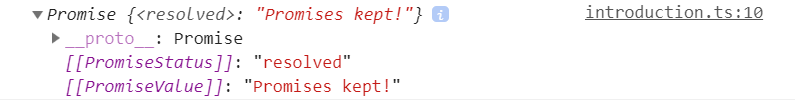
\includegraphics[width=12cm]{promise-beispiel-1}
\caption{}
\end{figure}

\noindent
Der Initialstatus eines Promise wird im nächsten Beispiel verdeutlicht:

\begin{figure}[H]
\begin{lstlisting}[basicstyle=\small]
export interface FakeHttpResponse {
    code: string;
    message: string;
}

const pendingPromise = new Promise<FakeHttpResponse>((resolve, reject) => {
    setTimeout(() => {
        resolve({
            code: '200',
            message: 'Promise kept!'
        });
    }, 10 * 1000);
});

console.log(pendingPromise);
setTimeout(() => console.log(pendingPromise), 10 * 1000);
\end{lstlisting}
\end{figure}

\noindent
Im oberen Beispiel wird das Promise vorbehaltlos nach zehn Sekunden aufgelöst, solange ist der Status ausstehend (pending). Nachdem das Promise aufgelöst wurde, werden Status und Wert aktualisiert. Dabei können nicht nur primitive Typen wie number, boolean oder strings zurückgegeben werden, sondern auch Objekt-Typen und komplexe Typen. Mit anderen Worten: Promises sind generisch.

\begin{figure}[H]
\centering
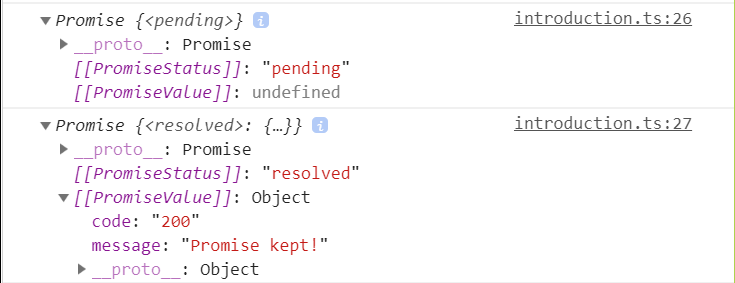
\includegraphics[width=12cm]{promise-beispiel-2}
\caption{Promise hat anfangs den Status \glqq{}ausstehend\grqq{}}
\end{figure}

\noindent
Wie man nun gesehen hat kann ein Promise Objekt den Status \textbf{pending}, \textbf{resolved} oder \textbf{rejected} haben. Im Status pending ist der Ausgang der Aktion noch ungewiss und deshalb der Promise-Wert undefined. Ändert sich der Status bzw. ist die Aktion zum Promise eingetroffen oder fehlgeschlagen, ist der Status \textbf{settled}. Grundsätzlich läuft ein Promise also vom pending in den settled Status. In der nächsten Sektion wird auf das Verarbeiten von Promises näher eingegangen.

\subsubsection{Verarbeiten von Promises}

Zur Wiederholung: Ein Promise-Objekt repräsentiert das eventuelle Eintreffen oder Fehlschlagen einer asynchronen Operation, einschließlich des entstandenen Wertes. Ein solches Objekt bietet \textbf{statische}- und \textbf{Prototyp}-Methoden. Die statischen Methoden können unabhängig von der Instanz aufgerufen werden, während die Prototyp-Methoden nur mit einer Promise Instanz aufrufbar sind. Eine oder mehrere der drei Prototyp-Methoden werden aufgerufen, wenn ein Promise in den settled Zustand eingetroffen ist:

\begin{description}

\begin{figure}[H]
\item \begin{lstlisting}[basicstyle=\small]
Promise.prototype.then(onFulfilled, onRejected)
\end{lstlisting}
\end{figure}

\begin{figure}[H]
\item \begin{lstlisting}[basicstyle=\small]
Promise.prototype.catch(onRejected)
\end{lstlisting}
\end{figure}
 
\begin{figure}[H]
\item \begin{lstlisting}[basicstyle=\small]
Promise.prototype.finally(onFinally)
\end{lstlisting}
\end{figure}
 
\end{description}


\noindent
Die untenstehende Grafik zeigt den Ablauf für das Eintreten der Events (onFulfilled, onRejected und onFinally) und wie man diese verarbeitet. Mit den Methoden \textbf{then()} und \textbf{catch()} werden auf eintretenden Aktionen reagiert. Diese Verarbeitungsmethoden werden aufgerufen wenn ein Promise in den settled Zustand angekommen ist. Im Erfolgsfall wird das Promise mit der then() Methode weiterverarbeitet. Im Fehlerfall hingegen wird die catch() Methode aufgerufen. Da beide Methoden ein Promise-Objekt zurückgeben, können Promises reibungslos aneinandergekettet werden. Wenn \textbf{finally()} an ein Promise Objekt angebunden wird, wird diese Methode in jedem Fall aufgerufen, unabhängig davon ob das Promise eingetroffen oder fehlgeschlagen ist.


\begin{figure}[H]
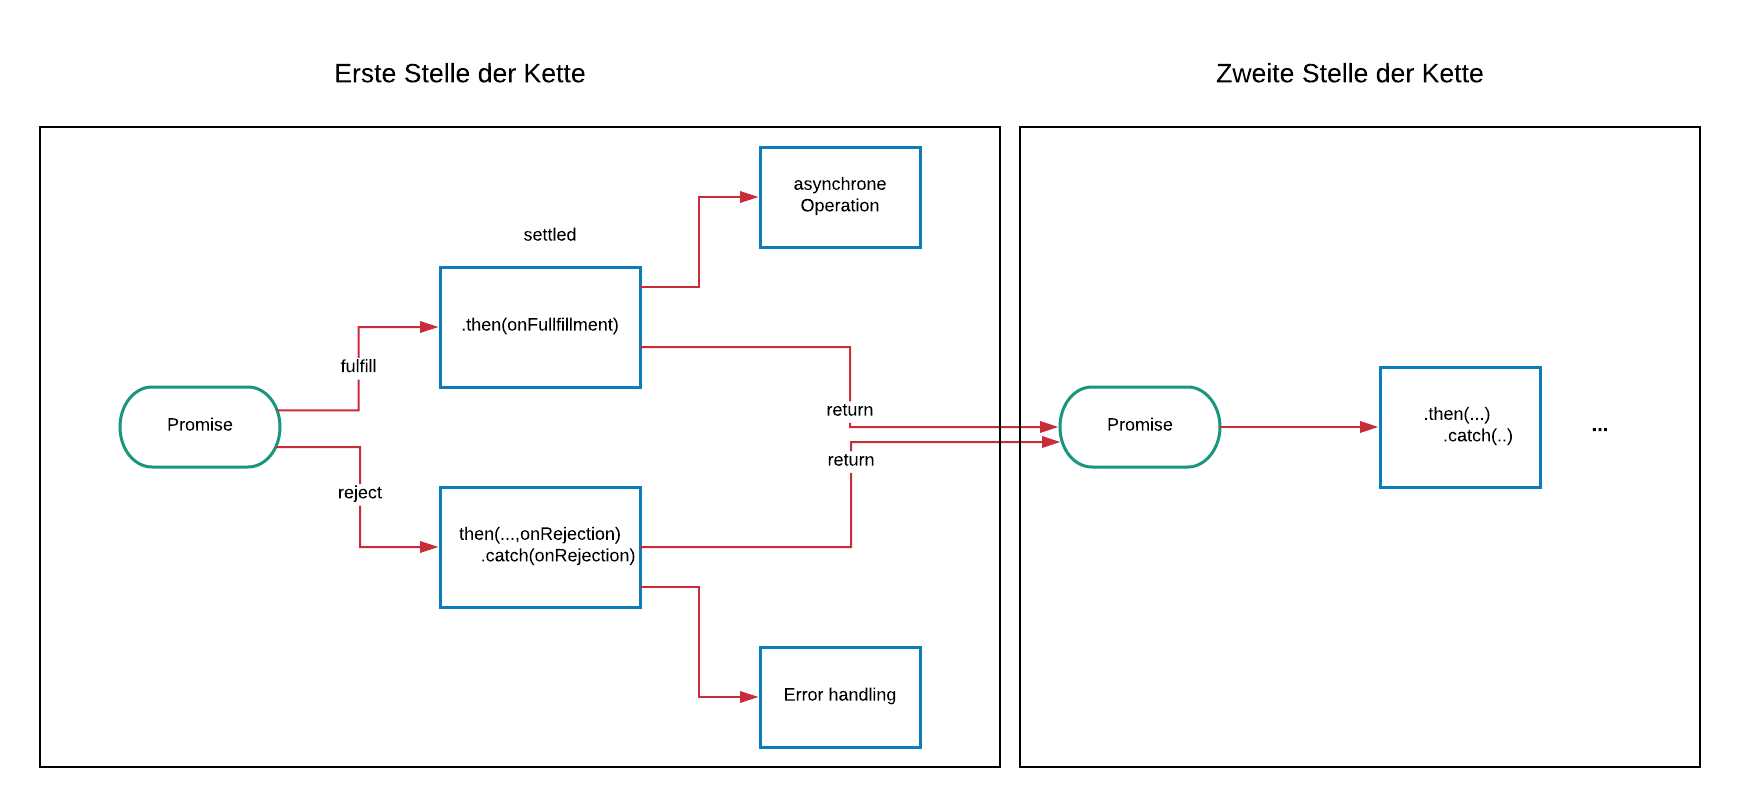
\includegraphics[width=13cm]{Promises-workflow}
\caption{Weiterreichung eines Promise-Objekts \cite{promise-executor}}
\end{figure}

\noindent
Promise-Fehlschläge können dabei auf zwei verschiedene Wege gefangen werden. Innerhalb der then()-Methode kann eine zweite, optionale Funktion für das \textbf{Nicht-Eintreffen} der Operation festgelegt werden. Ein Beispiel dafür wäre:

\begin{figure}[H]
\begin{lstlisting}[basicstyle=\small]
get('story.json').then((response) => {
  console.log('Success!', response);
}, (error) => {
  console.log('Failed!', error);
})
\end{lstlisting}
\caption{Error-Handling innerhalb der then()-Methode. \cite{callback-vs-promises}}
\end{figure}

\begin{figure}[H]
\begin{lstlisting}[basicstyle=\small]
get('story.json').then((response) => {
  console.log('Success!', response);
}).catch((error) => {
  console.log('Failed!', error);
})
\end{lstlisting}
\caption{Error-Handling mit der catch()-Methode. \cite{callback-vs-promises}}
\end{figure}

\noindent
Im Gegensatz zur oberen Variante führt die catch()-Methode keine zusätzlichen Operationen aus. Sie macht den Code lediglich semantisch lesbarer. Wichtig zu beachten ist, dass innerhalb einer Executor-Funktion \textbf{niemals} beide Argumente gemeinsam eintreffen können. Sie verhalten sich exklusiv. Deshalb ist das letztere Beispiel im Verhalten vergleichbar mit diesem Beispiel:

\begin{figure}[H]
\begin{lstlisting}[basicstyle=\small]
get('story.json').then((response) => {
  console.log('Success!', response);
}).then(undefined, (error) => {
  console.log('Failed!', error);
})
\end{lstlisting}
\end{figure}

\noindent
Der Unterschied ist minimal, aber extrem hilfreich. Promise-Fehlschläge gelangen bei der nächsten then()-Methode in den fehlgeschlagen Callback weiter oder in die catch Methode(,wenn vorhanden). Mit then(func1, func2) wird entweder die erste oder die zweite Funktion aufgerufen, aber niemals beide. Jedoch mit then(func1).catch(func2) werden beide Callbacks aufgerufen, sollte die erste Funktion fehlschlagen. Dies ist nur Möglich, da die Funktionen in unterschiedlichen Stellen der Verkettung liegen. Neben den Prototyp-Methoden gibt es, wie bereits erwähnt, die statischen Methoden. Diese bestehen aus vier Methoden:

\begin{itemize}
\item Promise.resolve()
\item Promise.reject()
\item Promise.race()
\item Promise.all()
\end{itemize}

\noindent
Die ersten beiden Methoden werden genutzt um einen eingetroffenen oder fehlgeschlagenen Promises zu simulieren:

\begin{figure}[H]
\begin{lstlisting}[basicstyle=\small]
const rejectedPromise = Promise.reject('I reject on purpose');

rejectedPromise.catch((err: string) => {
    console.log('Reason of failure: ' + err);
});
\end{lstlisting}
\end{figure}

\noindent
Diese Methoden können sich bei der Fehlersuche oder beim Testing als nützlich erweisen. Die anderen beiden Methoden helfen Promises leichter zu verarbeiten. Beispielsweise, wenn es darum geht mehrere Promises auszuführen, hat man entweder die Wahl die Promise-Verkettung zu nutzen oder die Promises in einem Array zu lagern und dann die nötigen Aktionen mit der Sammlung von Promises auszuführen. Im nächsten Beispiel wird die \textbf{Promise-Verkettung}, \textbf{Promise.all()} und \textbf{Promise.race()} gegenübergestellt. Zum Ausführen des Beispiels muss ../promises/stories.ts als Eingangsdatei konfiguriert werden.


\begin{figure}[H]
\begin{lstlisting}[basicstyle=\small]
export class HTTP {

    public makeRequest(url: string): Promise<any> {
        return new Promise((resolve, reject) => {
            const req = new XMLHttpRequest();
            req.open('GET', url);

            req.onload = () => {
                if (req.status === 200) {
                    this.fakeLatency()
                        .then(() => resolve(JSON.parse(req.response)));
                } else {
                    reject(Error(req.statusText));
                }
            };

            req.onerror = () => {
                reject(Error('Network Error'));
            };

            req.send();
        });
    }

    private fakeLatency() {
        return new Promise((resolve) =>
            setTimeout(resolve, 3000 * Math.random()));
    }
}
\end{lstlisting}
\end{figure}

\begin{figure}[H]
\begin{lstlisting}[basicstyle=\small]
export class Story {

    public static BASE_URL = 'https://jsonplaceholder.typicode.com/posts/';
    public spinnerElement: HTMLElement;

    public http: HTTP = new HTTP();

    constructor() {
       this.spinnerElement = Story.createElm('<svg>..</svg>');
    }

    public static createElm(innerHTML: string): HTMLElement {
        const div = document.createElement('div');
        div.innerHTML = innerHTML;
        document.body.appendChild(div);
        return div;
    }
    
    public getAllStories(): Promise<string> {
        return this.http.makeRequest(Story.BASE_URL);
    }

    public getChapter(chapter: number): Promise<string> {
        return this.http.makeRequest(Story.BASE_URL + chapter.toString());
    }
\end{lstlisting}
\end{figure}

\begin{figure}[H]
\begin{lstlisting}[basicstyle=\small]
    public spawn(content): void {
        if (content instanceof Array === false) {
            content = [content];
        }

        content.forEach(elm => {
            const snippet = document.createElement('div');
            snippet.innerHTML = '<h1>${elm.title}</h1>
                                 <div>
                                     <i>${elm.id}</i>
                                 </div>
                                 <p>${elm.body}.</p>';

            document.body.insertBefore(snippet, this.spinnerElement);
        });

    }

    public displayFinished(): void {
        this.spinnerElement.style.display = 'none';
        Story.createElement('All done!');
    }
}

const story = new Story();
\end{lstlisting}
\end{figure}

\noindent
Ähnlich wie im Beispiel des Callback-Kapitels wird von der REST-Api JSONPlaceholder Kapitel in die DOM geladen. In diesem Fall wurde hingegen das objektorientierte Paradigma gewählt. Die Klasse \textbf{HTTP} stellt mit makeRequest() eine Methode zur Verfügung, die eine Http-Anfrage gegen einen übergebenen Endpunkt macht. Mit der \textbf{Story} Klasse wird der Endpunkt der Datenabfrage als Klassenvariable definiert. Darüberhinaus werden mit getAllStories() und getChapter() die Methoden für die Abfrage definiert. Sollte ein Anwendungsfall sein, alle Kapitel anzuzeigen, würde der Code mit Promises so aussehen:

\begin{figure}[H]
\begin{lstlisting}[basicstyle=\small]
story.getAllStories()
    .then((response: XMLHttpRequestResponseType) =>
        story.spawn(response)
    )
    .finally(() =>
        story.displayFinished()
    );
\end{lstlisting}
\end{figure}

\noindent
Alle Kapitel werden mit einem Aufruf am Endpunkt angefragt. Ist das Promise in den settled Zustand angelangt, werden die Kapitel im Browser abgebildet. Als letzte Stelle der Kette wird mit finally der Lade-Icon ausgeblendet und eine Nachricht angezeigt, dass alle Stories abgebildet wurden. Sollte jedoch ein Anwendungsfall sein, dass nur drei Stories im Browser angezeigt werden sollen, könnte das wie folgt aussehen: 

\begin{figure}[H]
\begin{lstlisting}[basicstyle=\small]
story.getChapter(1).then(response1 => // (*)
    story.spawn(response1)
).then(() => // (**)
    story.getChapter(2).then(response2 => story.spawn(response2))
).then(() => // (***)
    story.getChapter(3).then(response3 => story.spawn(response3))
).finally(() =>  // (****)
    story.displayFinished()
);
\end{lstlisting}
\caption{Promise-Verkettung für sequentielle Ausführungen}
\end{figure}

\noindent
In diesem Fall werden nacheinander drei Kapitel angefragt und im Browser angezeigt. Da die Aufrufe im verketteten Konstrukt voneinander abhängig sind, addiert sich die Zeit die gebraucht wird, um ein Kapitel anzufragen und abzubilden. Die Idee dahinter ist, dass nach jedem Kapitelaufruf und -anzeige gewartet wird, bis dieser Vorgang abgeschlossen ist. Der Fluss sieht dabei so aus:

\begin{enumerate}
    \item Das initiale Promise wird aufgerufen und das Kapitel angezeigt. Das Promise gelangt in den settled Status. (*)
    \item Die nächste Stelle der Sequenz wird gestartet, diese endet erst, wenn die Operation innerhalb der then() Methode erfüllt ist (**)
    \item Die nächste Stelle der Sequenz wird initiiert...(***)
\end{enumerate}

\begin{figure}[H]
\centering
\includegraphics[width=12cm]{Promise-Verkettung-Stories.png}
\end{figure}

\noindent
Dieser Vorgang endet mit der finally() Verarbeitungsmethode. Zu beachten ist, dass das gesamte Verkettete Konstrukt in einem eigenen Thread läuft. Innerhalb dieses Threads verlaufen die Operationen jedoch sequentiell. Selbst bei einer weiteren Verzögerung der Kapitel innerhalb der Kette, wäre immer noch gewährleistet, dass die Kapitelaufrufe sequentiell ausgeführt werden:

\begin{figure}[H]
\begin{lstlisting}[basicstyle=\small]
story.getChapter(1).then((response1) => // (*)
    story.spawn(response1)
).then(() => // (**)
    new Promise(resolve => setTimeout(() => resolve(story.getChapter(2)), 5000))
        .then((response2) => story.spawn(response2))
).then() => ...
\end{lstlisting}
\end{figure}

\noindent
Das liegt daran, da die jeweilige then() Methode ein Promise-Objekt weiterreicht. Somit kann das nächste then() entsprechend nach entstandenem Status und Wert weiterarbeiten. Obwohl die Aufrufe in der Darstellung deutlich lesbarer als geschachtelte Callbacks sind, wird mit diesem Beispiel ebenfalls deutlich, dass bei Promise-Verkettungen der Code in die Länge gezogen wird. Zudem wird hier auch deutlich, dass asynchron Operationen ausgeführt werden. Eine zweite Variante ist, die Kapitel in einem Array Promise zu lagern und parallel mit Promise.all() auszuführen: 

\begin{figure}[H]
\begin{lstlisting}[basicstyle=\small]
const chapters: Array<Promise<void>> = [];

for (const n of [1, 2, 3]) {
    chapters.push(story.getChapter(n));
}

Promise.all(chapters).then((response) =>
    story.spawn(response)
).finally(() =>
    story.displayFinished()
);
\end{lstlisting}
\caption{Promise.all(iterable) bekommt ein iterierbares Objekt als Parameter übergeben}
\end{figure}

\noindent
Ein Promise.all() kann dabei abhängig vom Übergabeparameter verschiedene Rückgabewerte haben. Sollte das eingegebene iterable Argument leer sein, wird Promise.all() synchron erfüllt. Wenn das eingegebene iterable Argument keine Promises enthält, kommt ein asynchron eingelöstes Promise heraus. In allen anderen Fällen gibt ein Promise.all() ein einzelnes ausstehendes Promise zurück, dass eintrifft wenn alle Promises innerhalb des übergebenen Promise-Arrays eingetroffen sind. Die Rückgabewerte entsprechen dann der Reihenfolge der Promises, unabhängig von der Reihenfolge der Erfüllung.\cite{promise-all} Sollte ein Promise fehlschlagen, wird dieser ebenfalls fehlschlagen mit der Fehlernachricht des ersten fehlgeschlagenen Promise.\cite{promise-executor}\\

\noindent
Dabei ist zu beachten, dass die Promises parallel voneinander ausgeführt werden. Der unterschied der verketteten Variante zu Promise.all() liegt in der Art und Weise der Ausführung. Ein Promise.all() führt die Promises parallel aus und es löst sich nur so schnell auf wie das langsamste eintreffende Promise im iterable. Solange passiert nichts. In diesem Fall wird solange wird kein Kapitel in die DOM geladen, bis das langsamste Kapitel eingetroffen ist. In der verketteten Variante hingegen werden die Kapitel nacheinander im Browser geladen. Der Nutzer bekommt den Ladevorgang und das sequentiell laden der Kapitel mit. In der Praxis machen solche Kleinigkeiten eine nutzerfreundliche Applikation aus. 

\begin{figure}[H]
\centering
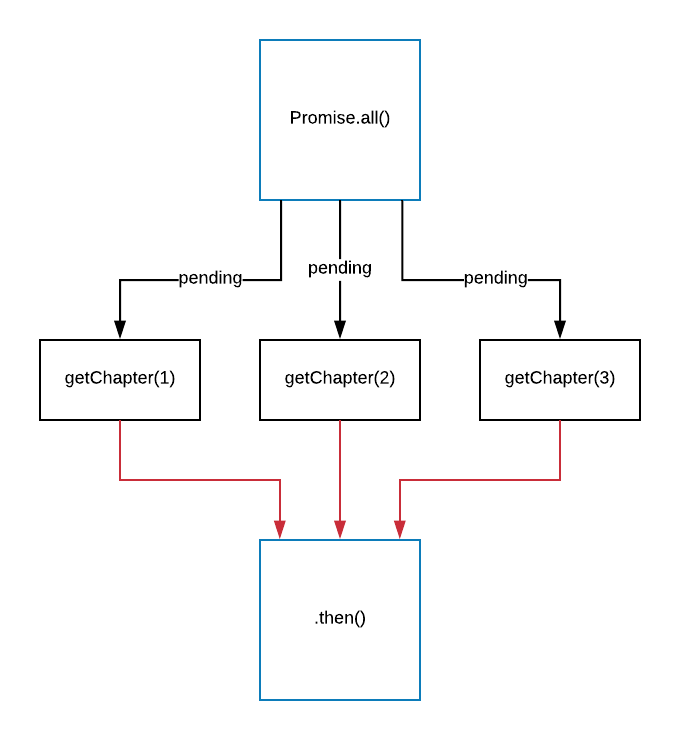
\includegraphics[width=7cm]{promise-all}
\caption{Die Nachrichten werden in der Reihenfolge ausgegeben, in der sie ins Array übergeben worden sind.}
\end{figure}

\noindent
Dagegen wird die nächste Methode verhältnismäßig seltener genutzt. Promise.race(iterable) gibt ein erfolgreiches oder fehlgeschlagenes Promise zurück, sobald eines der Promises in dem iterable erfolgreich war oder fehlgeschlagen ist, entsprechend mit dem Wert dieses Promises. Wenn das übergebene iterable leer ist, wird das Promise für immer im pending Status verharren.\cite{promise-race}

\begin{figure}[H]
\begin{lstlisting}[basicstyle=\small]
Promise.race(chapters).then((response) =>
    story.spawn(response)
).finally(() =>
    story.displayFinished()
);
\end{lstlisting}
\caption{Es wird schnellste ladende Kapitel angezeigt.}
\end{figure}

\subsection{Anti-Patterns und Best Practices}

Ob bei der Erstellung oder bei der Verarbeitung von Promises - Es gibt gewisse Ansätze nach denen man sich bei der Nutzung richten sollte. Ein negativ Beispiel für die Verarbeitung von Promises, wäre folgendes:

\begin{figure}[H]
\begin{lstlisting}[basicstyle=\small]
story.getChapter(1)
    .then((response1) => {
        story.spawn(response1);
        story.getChapter(2)
            .then((response2) => {
                story.spawn(response2);
                story.getChapter(3).then((response3) => {
                    story.spawn(response3);
                }).finally(() => {
                    story.spinnerElement.style.display = 'none';
                    story.displayFinished();
                });
            });
    });
\end{lstlisting}
\end{figure}

\noindent
Diese Methoden rufen ähnlich wie in Abbildung 13 drei Kapitel nacheinander auf. Obwohl sie im positiv Fall der API-Aufrufe die Kapitel sequentiell laden, wird hier komplett auf den Vorteil, den Promises gegenüber Callbacks bietet, verzichtet. Zudem ist die Ganze Kette davon abhängig, ob der erste Promise-Aufruf eintrifft. Hier wird keinerlei Möglichkeit gewährleistet ein Fehlschlag des ersten Aufrufs zu fangen ohne Code-Duplizierung. Solche ineinandergegliederte Promise-Verschachtelungen werden unter Entwicklern auch als \glqq{}Promise-Hell\grqq{} bezeichnet.
Mit dem ursprünglichen Beispiel ist es jedoch Möglich Fehler zwischen der Kette zu fangen:

\begin{figure}[H]
\begin{lstlisting}[basicstyle=\small]
story.getChapter(1)
    .then((response1) =>
        story.spawn(response1);
    )
    .catch((err) => ('Catched: ' + err))
    .then(() => story.getChapter(2)
        .then((response2) => 
            story.spawn(response2);
        ))
    ...
    \end{lstlisting}
\end{figure}

\noindent
Als Faustregel für Promises sollte beachtet werden, dass sie nur für einmalig auftretende asynchrone Events genutzt werden sollten. Der Verarbeitungsstatus eines Promise kann folgend sein:

\begin{itemize} 
\item Pending: Der Ausgang des Promises ist noch ungewiss.
\item Resolved: Die Aktion, die zum Promise verlief, ist eingetroffen.
\item Rejected: Die Aktion, die zum Promise verlief, schlug fehl.
\item Settled: Die Aktion ist entweder fehlgeschlagen oder eingetroffen - jedoch abgeschlossen.
\end{itemize}

\noindent
Beim erstellen einer Promise Instanz werden zwei Callback Funktionen als Argument angenommen. Resolve() wird mit der then() Methode verarbeitet und reject() mit der catch() Methode gefangen. Finally() kann unabhängig vom Eintreffen oder Fehlschlagen einer Operation genutzt werden. Der zurückgegebene Typ einer Promise Methode ist immer ein Promise-Objekt. Aufgrund dessen lassen sich Promises leicht verketten. Promises bieten mit Promise.all() und Promise.race() Hilfemethoden an, um mehrere Promises leichter zu verarbeiten.





\section{Async await}
Wenn es um das Verarbeiten von asynchronen Operationen geht, sind Promises ein erheblicher Fortschritt im Vergleich zum Callback Prinzip. Jedoch wurde ein grundlegendes Problem noch nicht gelöst: Mit der Nutzung von Promises ist der Code immer noch geschachtelt. Das liegt daran, da Verarbeitungsmethoden wie then() oder catch() weitere Callback Funktionen als Argument annehmen. Ziel ist es, asynchrone Aktionen so abzubilden, als ob diese synchron ausgeführt werden. 

\begin{figure}[H]
\begin{lstlisting}[basicstyle=\small]
module.exports = {
    mode: 'development',
    entry: './src/modules/async-await/introduction.ts',
    ...
}
\end{lstlisting}
\caption{Die webpack.config.js sollte im Folgenden als Eingangspunkt die ../async-await/introduction.ts Datei annehmen.}
\end{figure}

\begin{figure}[H]
\begin{lstlisting}[basicstyle=\small]
const hello: Promise<string> = new Promise(resolve =>
    setTimeout(() => resolve('Hello'), 1000));
    
const world: string = 'World';

hello
    .then(value => console.log(value, world));
\end{lstlisting}
\caption{Umsetzung mit einem Promise.}
\label{Promise-comparison-async-await}
\end{figure}

\noindent
Da Promises selbst Rückruffunktionen nutzen, wird einem schnell klar, dass hier eine asynchrone Aktion stattfindet. Mit der Erscheinung von Ecmascript 2017 gibt es nun die Möglichkeit asynchron operierenden Code lesbarer darzustellen. Dies wird mit dem \textbf{async await} Konstrukt bewerkstelligt. 

\subsection{Funktionsweise}

Async/Await sind Schlüsselwörter in Javascript, welche die asynchrone Programmierung wesentlich vereinfachen. Wenn vor einer Funktion das Schlüsselwort \textbf{async} steht bedeutet dies nur eins: Die Funktion gibt immer ein Promise zurück.

\begin{figure}[H]
\begin{lstlisting}[basicstyle=\small]
function hello() {
    return 'world';
}
\end{lstlisting}
\caption{Funktion gibt explizit und implizit ein String zurück.}
\end{figure}

\begin{figure}[H]
\begin{lstlisting}[basicstyle=\small]
async function hello() {
    return 'world';
}
\end{lstlisting}
\caption{Funktion gibt explizit ein String und implizit ein Promise\textless string\textgreater zurück.}
\end{figure}

\noindent
Der async Ausdruck an einer Funktion wandelt den Rückgabetyp T in ein Promise\textless T\textgreater{} um. Eine async Funktion kann zudem einen \textbf{await} Ausdruck enthalten. Mit await wird die Ausführung der Funktion pausiert bis das verwendete Promise eingetroffen ist. Daraufhin wird die Ausführung der Funktion mit dem zurückgegeben Wert des Promise fortgesetzt. Ein await ist nur innerhalb einer async Funktion valide einsetzbar. Das Beispiel in Abb. \ref{Promise-comparison-async-await} würde mit async await so aussehen:

\begin{figure}[H]
\begin{lstlisting}[basicstyle=\small]
const hello: Promise<string> = new Promise(resolve =>
    setTimeout(() => resolve('Hello'), 1000));
    
const world: string = 'World';

async function hello2() {
    const value = await hello;
    console.log(value, world);
}

hello2();
\end{lstlisting}
\caption{Umsetzung mit async await.}
\end{figure}

\noindent
Wie man sehen kann wird an dem await Ausdruck eine Konstante gebildet um das Ergebnis weiterzuverwenden. Für den Promise Wert werden keinerlei Verarbeitungsmethoden mehr benötigt. Der await Ausdruck greift direkt auf den Wert zu. Obwohl es für gewöhnlich so beschrieben wird, dass await die Exekution der Funktion pausiert, sollte man daraus nicht schlussfolgern, dass die Funktion synchron operiert. In Wahrheit, bricht await den synchronen Fluss und jede nachfolgende Anweisung innerhalb der Funktion operiert asynchron. Das heißt ein await Ausdruck blockiert nicht den synchronen Fluss von Javascripts Interpreter. Sie lässt das Ausführungsmodell asynchron agieren.

\begin{figure}[H]
\begin{lstlisting}[basicstyle=\small]
async function fn() {
    const result = await Promise.resolve('foo');
    console.log(result);
}

fn();
console.log('bar');
// bar
// foo
\end{lstlisting}
\caption{In diesem Fall wird bar vor foo angezeigt.}
\end{figure}

\noindent
Promise.resolve() und Promise.reject() sind weitere statische Promise Methoden, die ein neues Promise erstellen, dass entweder eintrifft oder fehlschlägt. Await stoppt die weitere Ausführung des Funktionsrumpfes, bis das Promise in den settled Zustand angelangt ist. Aber diese Auflösung findet erst statt, wenn der aktuelle Call stack vollständig verarbeitet wurde. Dieses Konzept wird auch \textbf{run to completion} genannt. Die Stärke von async await ist die Syntax. Eine Applikation, die von asynchronen Operationen getrieben ist, kann nun in der Code Struktur synchron abgebildet werden. 

\subsection{Error Handling}
Wenn ein Promise eintrifft, liefert der await Ausdruck das Ergebnis zurück. Hingegen wird bei einem Promise Fehlschlag ein Error geworfen, ähnlich wie bei einem \textbf{throw} Ausdruck. Wie in Java oder Swift gibt es auch in Javascript ein \textbf{try-catch} Block. Wenn ein Promise fehlschlägt, kann daraufhin mit dem catch Block der Fehler gefangen werden. Code-technisch würde dies so aussehen: 

\begin{figure}[H]
\begin{lstlisting}[basicstyle=\small]
async function fakeError() {
    try {
        const promise = await Promise.reject('Error');
        console.log(promise);
    } catch (error) {
        console.log('Upps: ', error);
    }
}

fakeError();
\end{lstlisting}
\caption{Es wird niemals console.log(promise) ausgeführt, da innerhalb des await Konstrukts eine Exception geworfen wird.}
\end{figure}

\noindent
Um sich ein besseres Bild von der Nützlichkeit von async await zu machen, werden die Kapitelaufrufe in der Promise Sektion mit async await nachgestellt. 

\begin{figure}[H]
\begin{lstlisting}[basicstyle=\small]
module.exports = {
    mode: 'development',
    entry: './src/modules/async-await/stories-usage.ts',
    ...
}
\end{lstlisting}
\caption{Vor dem Ausführen der Beispiele sollte die ../async-await/stories-usage.ts als Eingangsdatei definiert werden.}
\end{figure}

\begin{figure}[H]
\begin{lstlisting}[basicstyle=\small]
const story = new Story();

async function getFirstSections() {
    try {
        for (const n of [1, 2, 3]) {
            story.spawn(await story.getChapter(n));
        }
    } finally {
        story.displayFinished();
    }
}
\end{lstlisting}
\caption{Die Methode verhält sich genau so wie in Abb. \ref{Promises-sequential-calls}}
\end{figure}

\noindent
Ohne jegliche Verkettung wird mit dem await Konstrukt auf die Promise Auflösung gewartet und der entstandene Wert als Parameter in der Methode spawn() übergeben. Daraufhin wird weiter in der Schleife iteriert. Zudem bietet der try-catch Block auch finally an. Unabhängig vom Ausgang des try-catch wird im finally Block Code ausgeführt.

\subsection{Einsetzen wenn sinnvoll}

Beim Einsetzen von async await muss sich vor Augen geführt werden, wann ein Einsatz als solches Sinn ergibt. Kommt man wieder zum Anwendungsfall, man möchte die ersten drei Kapitel parallel in die DOM laden, würde der Code hierfür so aussehen:

\begin{figure}[H]
\begin{lstlisting}[basicstyle=\small]
async function getFirstSectionsInParallel() {
    try {
        const promises = [];

        [1, 2, 3].forEach(n => promises.push(story.getChapter(n)));

        story.spawn(await Promise.all(promises));
    } finally {
        story.displayFinished();
    }
}

getFirstSectionsInParallel();
\end{lstlisting}
\caption{Async await nutzt intern Promise Objekte.}
\end{figure}

\noindent
Wie man sehen kann gibt es keinen großen Mehrwert innerhalb der async await Exekution im Vergleich zur Abbildung \ref{Promise-all-example}. Beim übergeben der Promises in einem Array sind alle im pending Zustand. Erst mit await Promise.all(iterable) wird parallel auf die Auflösung der Promises gewartet. Die Stärke von async await kommt erst dann zur Geltung, wenn mehrere asynchrone Operationen sequentiell ausgeführt werden müssen. Als Faustregel kann festgelegt werden, dass async Funktionen ein Promise-Objekt zurückgeben. Selbst wenn explizit ein anderer Typ angegeben wird, stellt async sicher, dass dieser Typ immer ein Promise ist. Ein await Ausdruck pausiert die Ausführung einer async Funktion, bis die blockierende Aktion eingetroffen ist. Dabei können mehrere awaits innerhalb einer async Funktion definiert werden. Um Fehlschläge zu fangen sollte Javascripts try-catch Block angewendet werden. Es sollte unterschieden werden, ob der Code sequentiell oder parallel ausgeführt werden soll. Wenn asynchrone Aktionen parallel voneinander ausgeführt werden, kann man auf die Nutzung von async await verzichten.

\subsection{Fazit}

Mit dem Ansatz der Callbacks war es in Javascript erstmals möglich asynchrone Operationen sequentiell zu verarbeiten. Callbacks sind leicht zu verstehen, jedoch werden sie ineinandergeschachtelt schnell chaotisch und schwer nachzuvollziehen. Entwickler neigten dazu Libraries für asynchrone Verarbeitung zu nutzen wie:

\begin{center}
\begin{tabular}{ l c c r }
  Q & when & WinJS & RSVP.js\\
\end{tabular}
\end{center}

\noindent
Durch die Einbindung dieser Libraries konnte man in Javascript Promises nutzen. All diese externen Libraries teilen die gleiche Anatomie eines Promises und verhalten sich nach dem Standard \textbf{Promises/A+}\cite{promises-a+}. Promises wurden mit der Zeit immer beliebter. Sogar so beliebt, dass sie seit der Ecmascript-2015 Version rein nativ nutzbar sind. Mit der Einführung von async await war es sogar erstmals möglich asynchron operierenden Code übersichtlich abzubilden. Ganz ohne Verschachtelung wurde blockierender Code aufgelöst und in der nächsten Anweisung vorrangeschreitet. All diese Ansätze haben Eines gemeinsam: Beim Aufruf werden sie nur einmal verarbeitet. Wenn man mithilfe eines Promise ein Endpunkt-Aufruf macht und dieser eintrifft, ist es irrelevant, ob der Endpunkt nach zehn Sekunden nicht mehr erreichbar ist. Der Aufruf wurde bereits erfolgreich durchgeführt und das Ergebnis fertig verarbeitet. Mit Observables wird in der nächsten Sektion ein komplett neues Vorgehensmodell vorgestellt. Sie haben ein Strom-basiertes Verhalten, dass kein, ein oder multiple Werte mit der Zeit ausgeben. Dieser Ansatz unterscheidet sich grundlegend von den Bisherigen.

\section{RxJS: Reactive Extensions For JavaScript}
Rx ist eine Library, die für zahlreiche Programmiersprachen zur Verfügung gestellt wird. Diese finden sowohl in der Frontend als auch in der Backend-Implementierung Anwendung. In dieser Arbeit wird der Fokus auf RxJS geworfen. Diese Library ist eine Erweiterung speziell für Javascript/Typescript. RxJS erlaubt es mit Hilfe von Observable-Sequenzen Event-basierte Programme zu erstellen. Dabei wird dieser Ansatz auch als reactive Programming definiert. Neben der Kernfunktionalität von Observables werden auch Subjects und Schedulers geboten. Sollte man von reactive Programming noch nichts gehört haben, dann wird die größte Herausforderung sein \glqq{}reactive\grqq{} zu denken.

\subsection{Reactive Programming}
Im Kern ist reactive Programming ein Programmierparadigma. Im \textbf{reaktiven Manifest}, zu finden unter

\begin{center}
\url{https://www.reactivemanifesto.org/de},
\end{center}

\noindent
wird bereits beschrieben, dass Reactive Programming als Programmierung mit asynchronen, immutable Streams von Events bezeichnet wird. Laut der offiziellen Dokumentation richtet sich ReactiveX nach dem Beobachter-Muster (engl. Observer-Pattern). Das Observer-Pattern ist ein Entwurfsmuster, in der Änderungen eines Objektes (Subjects genannt) an einer Liste abhängiger Strukturen weitergereicht wird. Diese abhängige Strukturen (Observers) werden bei jeder Zustandsveränderung informiert. Eine Veränderung eines Objekts kann hierbei gleichgesetzt werden mit neuen Wert innerhalb eines Datenflusses. Als Beispiel für eine reaktive Anwendung kann Excel genommen werden. Ändert man einen Wert in einer Zelle, ändert sich auch der Wert in der Summenzelle. Die Zelle, deren Wert geändert wurde, löst ein Event aus, den die Summen-Zelle empfängt. Daraufhin findet eine Neuberechnung statt.\cite{reactive-programming-beispiel} Datenflüsse können aus verschiedensten Operationen entstehen wie z.B. Klick-Events, Variablen, Cache etc. Als Observer kann man sich in diesem Datenfluss einhängen und entsprechend reagieren.\cite{rx-intro} Rx bietet eine enorme Menge an Funktionen diese Datenflüsse zu bearbeiten/manipulieren (siehe Sektion Operatoren). Diese Operatoren komplett abzudecken wird in dieser Arbeit unmöglich sein, jedoch wird nach dem behandeln dieses Kapitels ein gewisses Grundverständnis für neue Operatoren entstehen und wie diese in Folge anzuwenden sind. Die grundlegenden Konzepte, um asynchrone Events in RxJS zu steuern, sind:

\begin{itemize}
    \item Observable: Repräsentiert die Idee einer abrufbaren Sammlung, in der zukünftige Werte oder Events gelagert sind.
    \item Observer: Eine Sammlung von Callbacks die, die  aus dem Observable-Stream gelieferten Werte, abrufen.
    \item Subscription: Repräsentiert das Aufrufen eines Observable.
    \item Operators: Funktionen, die das Verhalten von Observable-Streams beeinflussen.
    \item Subjects: Eventgeneratoren, die Events an zuhörende Observer zurückgibt. Im Gegensatz zu Observables, sind Subjects standardmäßig multicasting fähig.
    \item Schedulers: Steuerungsmechanismen die bestimmen, wann eine Subscription startet und wann Werte aus dem Stream an die Observer übermittelt werden.
\end{itemize}

\subsection{Observables}

Observables sind eine träge Sammlung von multiplen Werten. Sie füllen den fehlenden Platz in der unten stehenden Tabelle:

\begin{center}
    \begin{tabular}{| l | l | l |}
    \hline
    & \textbf{Einzelne-} & \textbf{Multiple Werte} \\ \hline
    \textbf{Pull/synchron} & Funktionen & Iterables (Arrays, Strings, ...) \\ \hline
    \textbf{Push/asynchron} & Promises & Observables  \\ \hline
    \end{tabular}
\end{center}

\noindent
Das Push- und Pull-Prinzip beschreibt dabei wie ein Datenproduzent mit dem Datenverarbeiter kommuniziert. In \textbf{Pull-Systemen} bestimmt der Verarbeiter, wann die Daten vom Ersteller angenommen werden. Der Ersteller selbst weiß nicht wann die Daten angefragt werden. Jede Javascript Funktion unterliegt einem Pull-System. Die Funktion ist ein Verarbeiter von Daten und diese kann im Code jederzeit abgerufen werden.\\

\noindent
Das \textbf{Push-Prinzip} wird im nächsten Beispiel deutlich. Vor dem Ausführen des Beispiels muss folgend konfiguriert werden:

\begin{center}
     async-patterns$\,\to\,$ webpack.config.js
\end{center}

\begin{figure}[H]
\begin{lstlisting}[basicstyle=\small]
module.exports = {
    mode: 'development',
    entry: './src/modules/rxjs/observable-introduction.ts',
    ...
}
\end{lstlisting}
\end{figure}

\begin{figure}[H]
\begin{lstlisting}[basicstyle=\small]
const alias: Observable<number> = RxJS.Observable.create((observer) => {
    observer.next(1);
    observer.next(2);
    observer.next(3);
    setTimeout(() => {
        observer.next(4);
        observer.complete();
    }, 1000);
});

console.log('Before subscribe');
alias.subscribe({
    next: x => console.log('Value: ' + x),
    error: err => console.error('Error occurred: ' + err),
    complete: () => console.log('Done!'),
});
console.log('After subscribe');
\end{lstlisting}
\caption{Observable verhalten sich sowohl synchron als auch asynchron.}
\end{figure}

\noindent
Das Observable-Objekt repräsentiert eine Kollektion die Werte zu seinen Beobachtern liefert. In diesem Beispiel wird ein Observable erstellt, dass sofort (synchron) die Werte 1, 2 und 3 produziert, sobald die Subscription gestartet wird. Der vierte Wert wird asynchron übermittelt und das Observable daraufhin geschlossen. Wichtig ist, dass man sich ein Observable-Stream nur mit der subscribe()-Methode anschließen kann. Die Konsole gibt die Werte in folgender Reihenfolge aus:

\begin{figure}[H]
\begin{center}
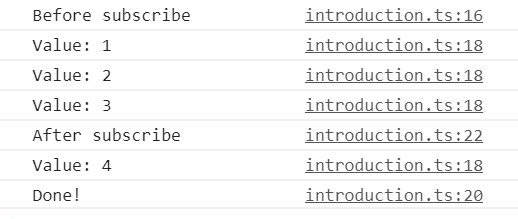
\includegraphics{observable-create-console}
\end{center}
\end{figure}

\noindent
Bei einer Subscription können drei verschiedene Events auftreten und somit drei verschiedene Funktionen aufgerufen werden:

\begin{itemize}
\item next: () =\textgreater Wenn ein Wert ausgegeben wird,
\item error: () =\textgreater Wenn ein Fehler ausgegeben wird,
\item complete: () =\textgreater Wenn sich der Stream schließt.
\end{itemize}

\noindent
In Push-Systemen steuert der Datenproduzent, wann die Daten an die Zu-hörenden übermittelt werden. Der Datenverarbeiter weiß hingegen nicht, wann die Daten ankommen. Promises sind ein typisches Beispiel für Push-Systeme. Ein Promise (Produzent) übermittelt einen eingetroffenen Wert an angeschlossene Callbacks (Verarbeiter). Ungleich wie mit Funktionen bestimmen Promises, wann die Werte an die Callbacks weitergereicht wird. Observables zählen zu einem neuen Push-System in Javascript. Im Gegensatz zu Promises emittieren Observables multiple Werte in Form von Streams. Zur Unterscheidung:

\begin{itemize}
\item Eine Funktion ist eine träge ausführende Operation, die beim Abruf ein Wert synchron zurückgibt.
\item Ein Promise ist eine Operation die einen eventuell eintreffenden oder nicht-eintreffenden Wert zurückgibt.
\item Ein Observable ist eine träge ausführende Operation, dass synchron oder asynchron keine oder potenziell unendlich viele Werte ab dem Zeitpunkt des Aufrufs zurückgibt.
\end{itemize}

\noindent
Hierbei stellt sich die Frage, was bedeutet träge? Träge Funktionen, im englischen auch als \textit{lazy Functions} bezeichnet, sind Funktionen die erst bei ihrem Aufruf Werte produzieren.\cite{lazy-functions}

\begin{figure}[H]
\begin{lstlisting}[basicstyle=\small]
function foo() {
    console.log('Hello');
    return 42;
}

const x = foo.call(this); // same as foo()
console.log(x);
const y = foo.call(this); // same as foo()
console.log(y);
\end{lstlisting}
\end{figure}

\begin{figure}[H]
\begin{lstlisting}[basicstyle=\small]
const foo = Rx.Observable.create((observer) => {
  console.log('Hello');
  observer.next(42);
});

foo.subscribe((x) => {
  console.log(x);
});
foo.subscribe((y) => {
  console.log(y);
});
\end{lstlisting}
\end{figure}

\noindent
Der Output bleibt immer derselbe:

\begin{figure}[H]
\begin{center}
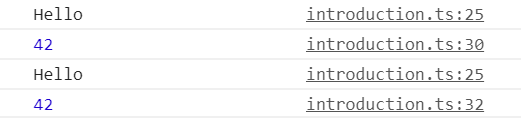
\includegraphics{observable-lazy-console}
\end{center}
\end{figure}

\noindent
Das liegt daran, da sowohl Funktionen als auch Observables träge sind. Die Operationen innerhalb beider Typen findet erst beim Aufruf statt. Mit anderen Worten: Das starten einer Subscription ist analog zum Aufruf einer Funktion. Entgegen der Annahme, dass Observables ausschließlich asynchron operieren, können diese ebenfalls synchron Werte ausgeben (siehe Abb. 25).
Der Hauptpunkt in dem Observables sich von Funktionen unterscheiden ist, dass Observables mehrere Werte (mit der Zeit) emittieren können. Innerhalb einer Funktion ist es nicht Möglich zwei return Ausdrücke einzubauen, die zusammen ausgegeben werden.

\subsubsection{Anatomie eines Observable}
Observables werden entweder mit der create Methode, mit einer Observable-Instanz oder mit der Hilfe eines Observable-Operators \textbf{erstellt}. Der Datenfluss wird an den Observern mit der subscribe()-Methode \textbf{überreicht}. Letzteres kann ein Observable \textbf{abgesetzt} werden.

\subsubsection{Observables erstellen}

\begin{figure}[H]
\begin{lstlisting}[basicstyle=\small]
const randomNumber = new Observable<number>(observer => {
    observer.next(Math.random());
});
\end{lstlisting}
\caption{Instantiierung eines Observables, als Parameter wird ein Callback angenommen.}
\end{figure}

\noindent
Die statische Methode Observable.create() ist ein alias ist zum Konstruktor-Aufruf. Für gewöhnlich werden jedoch sog. \textit{creation operators} wie \textbf{of}, \textbf{from}, \textbf{interval} etc. angewendet, um Observables zu erstellen. Im nächsten Abschnitt werden die verschiedenen Observable-Typen gegenübergestellt.

\subsubsection{Datenfluss überreichen}

Beim Aufruf der subscribe()-Methode überreicht der Datenproduzent ein eigenständigen Datenfluss an die Observer. Das hat zur Folge, dass mehrere Observer sich dem gleichen Observable anschließen und dennoch unterschiedliche Werte bekommen können.

\begin{figure}[H]
\begin{lstlisting}[basicstyle=\small]
const randomNumber = new Observable<number>(observer => {
    observer.next(Math.random());
});

randomNumber.subscribe(value =>
    console.log('1st subscription emits: ', value));
randomNumber.subscribe(value =>
    console.log('2nd subscription emits: ', value));
\end{lstlisting}
\end{figure}

\begin{figure}[H]
\begin{center}
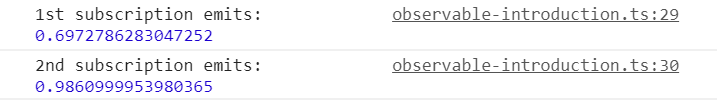
\includegraphics[width=12cm]{unicasting-observables}
\end{center}
\end{figure}

\noindent
Das Ergebnis sind zwei verschiedene Werte, bei zwei Subscriptions an einem Observable. Diese Eigenschaft wird als \textbf{unicasting} bezeichnet. Das ist nur Möglich, da die Funktion random() erst dann aufgerufen wird, wenn ein Observable mit der subscribe()-Methode aufgerufen wird. Somit hat jede Subscription einen eigenen Datenproduzent. Es gibt nun mehrere Möglichkeiten, dass sich Observers den gleichen Datenfluss teilen. Eine Möglichkeit wäre, den Datenproduzent außerhalb des Observable auszulagern. 

\begin{figure}[H]
\begin{lstlisting}[basicstyle=\small]
const dataProducer: number = Math.random();
const randomNumber = new Observable<number>(observer => {
    observer.next(dataProducer);
});

...
\end{lstlisting}
\end{figure}

\noindent
Eine elegantere Variante, wäre ein Operator anzuwenden, der den zuletzt eingetretenen Wert an die verschiedenen Observer teilt:

\begin{figure}[H]
\begin{lstlisting}[basicstyle=\small]
const multicast = randomNumber.pipe(shareReplay());

multicast.subscribe(value =>
    console.log('1st subscription emits: ', value));
multicast.subscribe(value =>
    console.log('2nd subscription emits: ', value));
\end{lstlisting}
\end{figure}

\noindent
Nun können multiple Subscriptions am Observable die gleiche Sequenz empfangen, da shareReplay() dafür sorgt, dass der Datenproduzent nur einmal aufgerufen werden kann und weitere Subscriptions sich diesen Datenproduzenten teilen. Diese Eigenschaft wird auch als \textbf{multicasting} bezeichnet. Das Ergebnis sieht wie folgt aus:

\begin{figure}[H]
\begin{center}
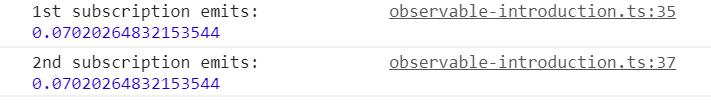
\includegraphics[width=12cm]{multicasting-observables}
\end{center}
\end{figure}

\noindent
Wenn Werte eines Streams erst beim Aufruf einer Subscription entstehen, handelt es sich hierbei um \textbf{cold Observables}.\cite{hot-vs-cold} Dies ist in jedem der oben angeführten Beispielen der Fall. Um auf die oben angeführte These zurück-zukommen, dass Observables träge sind, war dies zwar zum Einstieg in die Thematik hilfreich, aber nur die halbe Wahrheit. Observables können Werte emittieren auch ohne der subscribe()-Methode. Das bedeutet es werden Werte ausgestoßen, unabhängig davon ob eine Subscription stattfindet oder nicht. Hierbei würde es sich um ein \textbf{hot Observable} handeln. Um einen besseren Einblick zu bekommen, wird ein Observable erstellt, dass unendlich viele Werte ausstößt.

\begin{figure}[H]
\begin{lstlisting}[basicstyle=\small]
const infinite = RxJS.interval(1000).pipe(publish()) as ConnectableObservable<number>;
infinite.connect();

setTimeout(() =>
    infinite.subscribe(v => console.log('1st subscriber:', v)), 2000);
setTimeout(() =>
    infinite.subscribe(v => console.log('2nd subscriber: ', v)), 3000);
\end{lstlisting}
\end{figure}

\noindent
Die statische Methode interval() erstellt ein Observable, dass aufsteigend Nummern ausgibt innerhalb eines festgelegten Intervalls. Der Startindex ist 0. Die publish()-Funktion sorgt dafür, dass der Datenproduzent an die verschiedenen Subscriptions geteilt wird. In diesem Fall wird das Observable auch in einem \textbf{connectable Observable} umgewandelt. Das heißt es werden erst Werte innerhalb der Sequenz emittiert, sobald die entsprechende connect()-Methode am Observable aufgerufen wird.\\

\begin{figure}[H]
\begin{center}
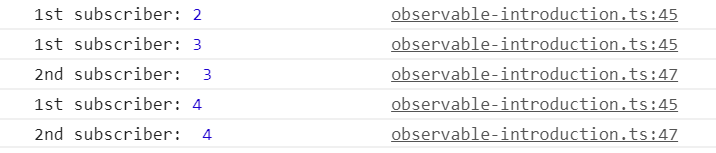
\includegraphics[width=12cm]{hot-observable}
\end{center}
\end{figure}



\noindent
Wie man nun gesehen hat hängt es vom Observable ab, wann die Sequenz von Werten emittiert werden. Ein hot Observable könnte Werte ausstoßen, sobald es erstellt wird. Und deshalb könnten Observers, die sich später am Observable-Stream einhängen, Werte zwischenzeitlich verpassen. Wenn der gleiche Datenproduzent über verschiedene Subscriptions genutzt wird, ist dies ebenfalls ein Indikator dafür, dass es sich um ein hot Observable handeln könnte. Ein cold Observable dagegen wartet mit dem emittieren der Werte, bis eine Subscription eines Observers stattgefunden hat. Dieser Observer empfängt dementsprechend die gesamten Werte der Sequenz. In manchen Versionen von Rx gibt es auch die Bezeichnung connectable Observable. In solchen Fällen werden erst dann Werte emittiert, wenn die abhängige connect()-Methode aufgerufen wurde, unabhängig davon ob eine Subscription an dem Observable stattfindet oder nicht.\cite{hot-vs-cold-part-2}

\noindent
\begin{center}
***Hier fehlt noch ordentlich was.*** 
\end{center}


\subsection{Operatoren}
Wenn es um Operatoren geht, sind diese die wahre Stärke der Observables. Operatoren gibt es in verschiedenen Kategorien: Sie manipulieren das Stream-Verhalten oder bearbeiten die Werte innerhalb eines Streams. Eines haben Operatoren gemeinsam. Wenn ein Operator an einem Stream angewendet wird, wird ein neuer Stream erstellt. Das liegt daran, dass Streams an sich unveränderbar (engl. immutable) sind.
Mit der aktuell neuesten Version von RxJS (6) ist nur noch Möglich Operatoren innerhalb der pipe() Methode anzuwenden.  ....

\subsubsection{Hot- vs. Cold-Observables}
\subsection{Subjects}
\subsubsection{Unicast vs. Multicast}










\section{Zusammenfassung}
\bibliography{references}

\end{document}
